% !TEX program = lualatex
%% ===================================================================
%% Taylor & Francis / STAM Methods manuscript template
%% All numerical values originate from paper/paper_data.json.
%% Compile with lualatex (temporary luatexja for Japanese query examples).
%% ===================================================================
\documentclass[twocolumn]{interact}

% Temporary: luatexja is required for Japanese NL query examples in tables.
% Remove before final submission to STAM Methods and translate those examples.
\usepackage{luatexja}
% Body text at 10pt (interact.cls default is 11pt).
\makeatletter
\renewcommand\normalsize{%
   \@setfontsize\normalsize{10}{12.5}%
   \abovedisplayskip 13\p@ \@plus2\p@ minus.5pt
   \abovedisplayshortskip \abovedisplayskip
   \belowdisplayskip 13\p@ \@plus2\p@ minus.5pt
   \belowdisplayshortskip\belowdisplayskip
   \let\@listi\@listI}
\makeatother
\normalsize
% Reduced page margins (interact.cls default: textwidth=34pc, textheight=650pt).
\geometry{margin=20mm}
\usepackage{url}
\usepackage{cite}
\usepackage{chngcntr}
\usepackage[hidelinks]{hyperref}
\setlength{\columnsep}{16pt}

\usepackage{graphicx}
\usepackage{multirow}
\usepackage{amsmath,amssymb,amsfonts}
\usepackage{xcolor}
\usepackage{siunitx}
\usepackage{longtable}
\usepackage{array}
\usepackage{float}
\usepackage{enumitem}
\usepackage{subcaption}
\usepackage{listings}
\usepackage{algorithm}
\usepackage{algpseudocode}
\usepackage{tabularx}
\usepackage{tikz}
\usetikzlibrary{arrows.meta,positioning,shapes.geometric,fit,calc,backgrounds}

% interact.cls redefines \toprule/\midrule/\bottomrule as \hline with extra \\
% which creates empty rows and bad spacing. Restore the original booktabs
% definitions (booktabs is already loaded by interact.cls).
\makeatletter
\def\toprule{\noalign{\ifnum0=`}\fi
  \@aboverulesep=\abovetopsep
  \global\@belowrulesep=\belowrulesep
  \global\@thisruleclass=\@ne
  \@ifnextchar[{\@BTrule}{\@BTrule[\heavyrulewidth]}}
\def\midrule{\noalign{\ifnum0=`}\fi
  \@aboverulesep=\aboverulesep
  \global\@belowrulesep=\belowrulesep
  \global\@thisruleclass=\@ne
  \@ifnextchar[{\@BTrule}{\@BTrule[\lightrulewidth]}}
\def\bottomrule{\noalign{\ifnum0=`}\fi
  \@aboverulesep=\aboverulesep
  \global\@belowrulesep=\belowbottomsep
  \global\@thisruleclass=\@ne
  \@ifnextchar[{\@BTrule}{\@BTrule[\heavyrulewidth]}}
\makeatother

\setlist{nosep,leftmargin=*}

\lstset{
  basicstyle=\ttfamily\footnotesize,
  breaklines=true,
  frame=single,
  language=SQL,
  keywordstyle=\color{blue}\bfseries,
  commentstyle=\color{green!50!black},
  stringstyle=\color{red!70!black},
  numbers=left,
  numberstyle=\tiny\color{gray},
  tabsize=2,
}

% =====================================================================


\begin{document}

\title{無機材料データベースの自然言語アクセス：\\
正確・保守可能・安全なデータ検索のためのText-to-SQL基盤}

\author{
\name{源 聡\textsuperscript{a}\thanks{CONTACT 源 聡. Email: minamoto.satoshi@nims.go.jp} and 末松 知恵\textsuperscript{a}}
\affil{\textsuperscript{a}Materials Data Platform, National Institute for Materials Science (NIMS), 1-1 Namiki, Tsukuba 305-0044, Ibaraki, Japan}
}

\twocolumn[{%
\maketitle
\begin{abstract}
密度汎関数理論（DFT）計算で得られた無機材料の組成・結晶構造・生成エネルギー・物性値は、OQMDなどのデータベースに正規化リレーショナルデータベース（RDB）として蓄積されている。正規化RDBでは情報が多数のテーブルに分かれて格納されるため、目的のデータを取り出すにはテーブル構造とSQLの理解が必要であり、これが材料研究者にとって利用の障壁となっている。本研究では、自然言語の質問文からSQLを自動生成するText-to-SQLパイプラインを、DFT計算データを格納した無機材料RDB向けに設計し、検証する。パイプラインは、材料用語をSQL条件へ対応付ける材料ドメイン辞書、関連テーブルの選択、類似質問とSQLの例（few-shot例）の検索、外部キー（FK）関係に基づくJOIN経路の制約、複数のSQL候補の生成と選択、実行前のSQL安全性検証（SQLGuard）と読み取り専用実行から構成される。これにより、「安定な化合物」「体積弾性率150 GPa以上」のような専門用語・物性条件を含む日本語の質問文から、複数テーブルにまたがる検索や、生成エンタルピーの参照状態補正のような多段計算を、研究者がSQLを書かずに実行できる。5プロトタイプ（L1$_2$/B2/NaCl/NiAs/BiF$_3$）・36テーブルの検証RDB上で245の自然言語クエリを評価した結果、行レベルの実行再現率は86.1\%であった（この値は期待される行の回収率であり、SQLの完全一致率ではない）。実装に関与していない共同著者が設計した100問、スキーマの異なる3種のRDBへの一般化試験、日英の質問文による評価の結果も報告する。各構成要素の寄与はablation study（構成要素を1つずつ外して性能変化を測る実験）と統計検定で評価した。本手法は辞書・few-shot例・FKメタデータの差し替えで他の正規化材料RDBへ適応できる。
\end{abstract}

\begin{keywords}
Text-to-SQL \; 無機材料データベース \; 自然言語インターフェース \; スキーマグラフ \; ドメイン特化辞書 \; 材料インフォマティクス
\end{keywords}
\vspace{1.5em}
}]

% =====================================================================
\section{はじめに}
\label{sec:introduction}

\paragraph*{無機材料研究におけるデータ探索の障壁}

密度汎関数理論（DFT）に基づく第一原理計算は、無機材料の結晶構造・全エネルギー・生成エネルギー・電子状態・弾性定数などを、実験を行わずに計算で求める手法である。OQMD~\cite{saal2013oqmd,kirklin2015oqmd}、Materials Project~\cite{jain2013mp}、AFLOW~\cite{curtarolo2012aflow}、NOMAD~\cite{draxl2019nomad}などのデータベースは、こうしたDFT計算の結果を数万から数十万件の規模で蓄積している。AtomWork-Adv~\cite{nims2018atomworkadv}のように文献由来の実験データを収録するデータベースもある。本研究が対象とするのは、このようなDFT計算由来の無機材料データを格納したデータベースである。

これらのデータは通常、正規化リレーショナルデータベース（RDB）に保存される。正規化とは、組成・結晶構造・安定性・物性値などの情報を種類ごとに別のテーブルに分け、テーブル間を外部キー（FK；他のテーブルの行を指す識別子列）で結びつける設計方針である。この設計では、1つの質問に答えるために複数のテーブルをJOIN（FKで結合）するSQLが必要になる。多くのデータベースはAPIも備えるが、APIは複数テーブルをまたぐ条件検索や統計処理には向かない。一方、RDBを直接利用するにはテーブル構造、FK関係、SQL構文の理解が必要であり、材料研究者にとって障壁となる。

共通APIであるOPTIMADE~\cite{andersen2021optimade}はフィルタ構文によるデータベース横断検索を提供し、対応データベースも増えている~\cite{evans2024optimade}。ただし、検索対象は各データベースが公開する共通スキーマの属性に限られ、RDB内部の正規化テーブルをまたぐJOINや集計の代わりにはならない。自然言語の質問文からSQLを自動生成できれば、材料研究者はテーブル構造を意識せずにデータを探索できる。

\paragraph*{Text-to-SQL技術と材料科学における現状}

自然言語の質問文からSQLを自動生成する技術をText-to-SQLと呼ぶ。この技術はSpider~\cite{yu2018spider}やBIRD~\cite{li2024bird}のベンチマーク（評価用の質問文とSQLの組）を中心に発展してきた。大規模言語モデル（LLM）を用いる手法として、DIN-SQL~\cite{pourreza2024dinsql}はスキーマリンク（質問文中の語をテーブル・カラムへ対応付ける処理）・分類・生成を分離したパイプラインを、DAIL-SQL~\cite{gao2023dail}は少数ショット例（プロンプトに含める質問文とSQLの例）の選択方法を提案した。RAT-SQL~\cite{wang2020ratsql}はスキーマ内の関係を考慮した符号化を、RESDSQL~\cite{li2023resdsql}はスキーマリンクと生成の分離を導入した。SchemaGraphSQL~\cite{safdarian2026schemagraphsql}はFK関係をグラフとして扱い、その上で経路探索を行う点で本研究に最も近い。

これらの手法は一般分野のベンチマークで評価されており、無機材料データベースのような特定分野のRDBでの効果は検証されていなかった。MatSciBERT~\cite{gupta2022matscibert}やMatBERT~\cite{walker2021matbert}は材料科学の文献テキスト向けの言語モデルであり、Text-to-SQLには適用されていない。MKNA~\cite{zhuang2026mkna}やOptiMat~\cite{hu2026optimat}はAPIを通じたアクセスを提供するが、正規化RDBに対してJOINを制御しながらSQLを生成する機能はない。SuperCon~\cite{ishii2023supercon}やPoLyInfo~\cite{ishii2024polyinfo}はRDF/SPARQL（グラフ形式のデータとその問い合わせ言語）に基づくため、既存のRDBに適用するにはデータ変換が必要である。また、LLMにテーブル定義だけを与えてSQLを生成させると、存在しないテーブルやカラムを参照したり、条件が不完全になったりする（定量値はセクション~\ref{sec:llm_only}、生成SQLの実例は補足資料~\ref{sec:sup_sql_examples}）。汎用LLMを材料分野の課題にプロンプトのみで適用した場合、幻覚や無効出力が多く、タスク固有の知識の導入が必要であることは物性予測でも報告されている~\cite{rubungo2025llmmatbench}。

\paragraph*{目的と貢献}

本研究の目的は、Text-to-SQL手法の一般的な性能比較ではない。DFT計算データを格納した無機材料RDBに対して、自然言語で問い合わせるための設計を提示し、再現可能な形で検証することである。対象とする分野特有の課題は次の3つである：
\begin{enumerate}
  \item ドメイン用語の曖昧さ：
    L1$_2$、$\gamma'$相、B2のような結晶構造名や物性用語はLLMの学習データに少なく、SQL条件への変換を誤りやすい。
  \item 複数テーブルJOINの複雑さ：
    正規化された材料RDBでは数十のテーブルをJOINする必要があり、LLMはFK関係に基づかない誤ったJOINを生成しやすい。
  \item 評価データの欠如：
    無機材料RDBにおけるText-to-SQLの標準評価ベンチマークは存在しない。
\end{enumerate}

本研究の貢献は4つある：
\begin{enumerate}[label=(\roman*)]
  \item 材料RDB Text-to-SQLのための設計原則：
    材料ドメイン辞書とfew-shot例による分野適応、FKグラフ上の貪欲最短経路連結（必要なテーブルをFK関係の最短経路で順につなぐ方法）によるJOIN制約、およびリランカー（複数のSQL候補から1本を選ぶ機構）を組み合わせたパイプラインを提案する。
  \item 多軸定量評価：
    L1$_2$を中心に5プロトタイプを含む36テーブル・総行数約2.2万行の検証RDB（設計はセクション~\ref{sec:evaluation}）に対し、245クエリを複数の指標（厳密な完全結果集合一致 / SELECT列精度 / JOIN一致率）で評価する。加えて、100クエリのサブセットで7条件$\times$5回のアブレーション（クエリ単位の対応あり検定とブートストラップ95\%信頼区間）、少数ショット例数$k$の感度、辞書サイズの感度、LLMモデル比較を行う。
  \item ドメイン知識の定量的効果：
    構成要素を外したときの低下幅（パーセントポイント；pp）で見ると、少数ショット例の寄与が最大（$-$16.1\,pp, $p<0.001$）で、材料辞書（$-$9.8\,pp, $p=1.0\times10^{-4}$）もHolm補正（複数の検定を同時に行う際のp値の補正）後も有意である。リランカーは$-$6.2\,ppで、未補正$p=0.0195$だがHolm補正後は有意でない。
  \item スキーマ一般化と言語依存性の検証：
    条件の異なる4種の一般化試験---A~同一スキーマ上の5プロトタイプ横断クエリ（主評価の部分集合の別ラン；100.0\%）、B~テーブル名・カラム名をOQMD風に変更したスキーマ（85.0\%）、C~名前をランダム化したスキーマ（80.0\%）、D~Materials Projectの実データを用いた別スキーマ（93.3\%）---を比較する。Aはスキーマの変更を含まず、DはMP専用のfew-shot例を用いるため、4条件は区別して解釈する（セクション~\ref{sec:transfer_eval}）。さらに、同一100クエリ・同一gold SQLで質問文の言語だけを日本語と英語で変えた比較と、翻訳を経ない英語25クエリにより、質問文の言語への依存性を検証する（セクション~\ref{sec:language_eval}）。
\end{enumerate}

% =====================================================================

\section{方法}
\label{sec:method}

\subsection{データベースと評価設計}
\label{sec:evaluation}  
\subsubsection{検証データベース}

DFT計算による無機材料データを格納する正規化RDBを想定し、L1$_2$型金属間化合物を題材とする検証RDBを構築した。組成・結晶構造・熱力学的安定性・電子構造・機械的特性・表面特性などの情報を36の正規化テーブル（うち1つはスキーマ初期化状態の管理表\texttt{schema\_initialization\_status}）と1つのビューに分けて配置し、材料エントリを表す\texttt{material\_entry}テーブルを中心にFK関係で周辺テーブルと接続する。主要テーブルの関係（ER図）を図~\ref{fig:er}に示す。テーブル36、ビュー1、\texttt{material\_entry} 1{,}559行、\texttt{composition} 3{,}029行、\texttt{calculated\_property} 4{,}410行、プロトタイプ5種などの統計は補足資料~\ref{sec:sup_method_details}の表~\ref{tab:db_stats}に示す。公開OQMDのデータモデル（少数の幅広いテーブルにエントリ情報をまとめる構成）との対応は補足資料の表~\ref{tab:schema_comparison}に示す。

\begin{figure*}[htbp]
\centering
\resizebox{0.9\textwidth}{!}{%
\begin{tikzpicture}[
  >=Stealth,
  every node/.style={font=\scriptsize},
  entity/.style={rectangle, draw, rounded corners=2pt,
    minimum height=0.6cm, minimum width=1.8cm, align=center,
    text width=1.8cm, font=\scriptsize},
  core/.style={entity, fill=blue!15, line width=0.8pt},
  prop/.style={entity, fill=green!12},
  master/.style={entity, fill=orange!15},
  junction/.style={entity, fill=yellow!15},
  electronic/.style={entity, fill=cyan!12},
  mechanical/.style={entity, fill=red!8},
  surface/.style={entity, fill=purple!10},
  phase/.style={entity, fill=teal!12},
  experiment/.style={entity, fill=pink!15},
  defect/.style={entity, fill=brown!12},
  fk/.style={->, thick, color=gray!60, >=Stealth},
  grouplabel/.style={font=\footnotesize\bfseries, text=gray!50},
]

% Row 0: Master Tables
\node[master] at (-6, 5.5) (sg) {space\_group\\{\tiny H-M, crystal sys}};
\node[master] at (-2, 5.5) (proto) {prototype\_\\definition\\{\tiny Strukturbericht}};
\node[master] at (2, 5.5) (elem) {element\\{\tiny Z, mass, $\chi$}};
\node[prop] at (5.5, 5.5) (eprop) {element\_property\\{\tiny property, value}};

% Row 1: Core entities
\node[core, minimum width=2.4cm, minimum height=0.8cm, line width=1.2pt,
      font=\scriptsize\bfseries] at (0, 3) (me) {material\_entry\\{\tiny (PK: entry\_id)}};
\node[core] at (-5, 3) (comp) {composition\\{\tiny element, fraction}};
\node[core] at (-2.5, 4.2) (struct) {structure\\{\tiny prototype, lattice}};
\node[core] at (2.5, 4.2) (ps) {phase\_stability\\{\tiny $E_f$, $E_{hull}$}};
\node[core] at (5, 3) (calc) {calculation\\{\tiny method, functional}};
\node[prop] at (8.5, 3) (cprop) {calculated\_property\\{\tiny name, value, unit}};

% Row 2: Application/Literature + Electronic
\node[master] at (-8, 1.5) (appdom) {application\_domain\\{\tiny domain, hierarchy}};
\node[junction] at (-5.5, 1.5) (matapp) {material\_\\application\\{\tiny relevance}};
\node[experiment] at (-8, 0) (litref) {literature\_\\reference\\{\tiny DOI, journal}};
\node[junction] at (-5.5, 0) (matref) {material\_reference\\{\tiny context}};

\node[electronic] at (5, 1.5) (bs) {band\_structure\\{\tiny gap, CBM, VBM}};
\node[electronic] at (8.5, 1.5) (dos) {density\_of\_states\\{\tiny DOS@$E_F$, metallic}};

% Row 3: Experimental + Mechanical
\node[experiment] at (-8, -1.5) (expmt) {experimental\_\\measurement\\{\tiny method, T, P}};
\node[experiment] at (-5.5, -1.5) (mprop) {measured\_property\\{\tiny name, value}};

\node[mechanical] at (1.5, 0) (elastic) {elastic\_tensor\\{\tiny $B$, $G$, $E$, $\nu$}};
\node[mechanical] at (5, 0) (mag) {magnetic\_property\\{\tiny $M$, ordering, $T_C$}};
\node[mechanical] at (8.5, 0) (therm) {thermal\_property\\{\tiny $\Theta_D$, $\kappa$, $C_v$}};

% Row 4: Synthesis/Defect + Surface
\node[defect] at (-8, -3) (synm) {synthesis\_method\\{\tiny name, category}};
\node[junction] at (-5.5, -3) (matsyn) {material\_synthesis\\{\tiny T, duration, atm}};
\node[defect] at (-2, -3) (deftype) {defect\_type\\{\tiny vacancy, antisite}};
\node[junction] at (1.5, -3) (matdef) {material\_defect\\{\tiny $E_f$, site}};

\node[surface] at (5, -1.5) (surf) {surface\_energy\\{\tiny $(hkl)$, $\gamma$, $\phi$}};
\node[surface] at (8.5, -1.5) (gb) {grain\_boundary\\{\tiny $\Sigma$, $E_{GB}$}};

% Row 5: Phase/Alloy
\node[phase] at (1.5, -4.5) (pde) {phase\_diagram\_entry\\{\tiny hull, decomp}};
\node[phase] at (5, -4.5) (alloy) {alloy\_system\\{\tiny name, components}};
\node[junction] at (8.5, -4.5) (ma_alloy) {material\_alloy\_\\system\\{\tiny phase, comp type}};
% FK矢印: コア -> material_entry
\draw[fk] (comp) -- (me);
\draw[fk] (struct) -- (me);
\draw[fk] (ps) -- (me);
\draw[fk] (calc) -- (me);

% FK: material_entryへの接続
\draw[fk] (matapp) -- (me);
\draw[fk] (matref) -- (me);
\draw[fk] (expmt.east) -- ++(1.5,0) |- ([yshift=-0.1cm]me.west);
\draw[fk] (bs) -- (me);
\draw[fk] (dos.south west) -- (me);
\draw[fk] (elastic) -- (me);
\draw[fk] (mag.north) -- (me);
\draw[fk] (therm.north west) -- (me);
\draw[fk] (surf.north west) -- (me);
\draw[fk] (gb.north) -- ([xshift=0.3cm]me.south east);
\draw[fk] (matsyn.north) -- ([xshift=-0.5cm]me.south);
\draw[fk] (matdef.north) -- ([xshift=0.2cm]me.south);
\draw[fk] (pde.north) -- ([xshift=-0.3cm]me.south);
\draw[fk] (ma_alloy.north west) -- (me);

% FK: 計算子の子供
\draw[fk] (cprop) -- (calc);
\draw[fk] (bs) -- (calc);
\draw[fk] (dos.west) -- (calc);
\draw[fk] (elastic.north east) -- (calc);
\draw[fk] (therm.north) -- (calc);

% FK: マスターテーブルの参照
\draw[fk] (eprop) -- (elem);
\draw[fk] (matref) -- (litref);
\draw[fk] (expmt) -- (litref);
\draw[fk] (matsyn) -- (synm);
\draw[fk] (matsyn) -- (litref);
\draw[fk] (matdef) -- (deftype);
\draw[fk] (matapp) -- (appdom);
\draw[fk] (ma_alloy) -- (alloy);
\draw[fk] (mprop) -- (expmt);
\draw[fk] (matdef.north west) to[bend right=15] (elem.south east);

% 自己参照FK
\draw[->, thick, color=red!60] (appdom.north) to[out=130,in=50,looseness=4]
  node[above, font=\tiny, text=red!60] {親} (appdom.north east);

% グループラベル
\node[grouplabel] at (-2, 6.3) {マスターテーブル};
\node[grouplabel] at (0, 4.8) {コアエンティティ};
\node[grouplabel] at (-7, -4.2) {合成/欠陥};
\node[grouplabel] at (7, -2.5) {表面/界面};
\node[grouplabel] at (5, -5.3) {相図/合金};
\node[grouplabel] at (-7, 2.5) {文献/応用};
\node[grouplabel] at (7, 2.5) {電子構造};
\node[grouplabel] at (5, -0.8) {機械的特性};

\end{tikzpicture}%
}% end resizebox
\caption{36テーブル検証データベースの主要テーブルのER図。
  コアテーブル（組成、構造、安定性など）はFK関係を介して中央の\texttt{material\_entry}に直接接続されている。
  計算された特性と電子構造には2つの経路がある：
  直接FKと\texttt{calculation}を介した経路である。
  矢印はFK参照の方向を示している。}
\label{fig:er}
\end{figure*}

格納データのうち、生成エンタルピー計算の参照状態に用いる純元素の参照エネルギーはOQMDのDFT計算値をそのまま用いた。それ以外の化合物データ（全エネルギー、生成エネルギー、格子定数、弾性率など）は、OQMDのデータ形式と値の範囲を参考にプログラムで生成した合成検証データであり、実在する化合物の計算結果ではない。キュリー温度、$\Sigma$粒界エネルギー、合成方法、文献参照など、OQMDにはないが一般の材料RDBが持つ属性も合成生成し、独立評価の磁気・熱特性および表面・粒界・欠陥カテゴリ（セクション~\ref{sec:independent_eval}）のクエリはこれらのテーブルを対象とする。合成データを用いる理由は、SQL生成の正否を判定するための正解（ゴールドSQLと期待結果）を、データの内容を完全に把握した状態で作成するためである。評価用SQLは平均3.4、最大6テーブルの結合と、多段階のCTE（共通テーブル式；中間結果に名前を付けて段階的に計算するSQLの構文）を要する。

\subsubsection{評価クエリ}
\label{sec:query_design}

主評価には245クエリの評価コーパス（Easy 43 / Medium 69 / Hard 69 / Very Hard 64；以下 Very Hard を VH と略記）を使用した。145クエリは著者が、100クエリは実装に関与していない共同著者が独立に設計した（後者の別ラン再評価はセクション~\ref{sec:independent_eval}）。245クエリは表~\ref{tab:main_partition}のとおり5群に重複なく分割される（著者設計145＝100+20+10+15）。このうち独立設計100・バリアントA 20・CTE 15（アブレーション用サブセット内の5＋ゼロショット10）の計135クエリは、セクション~\ref{sec:additional_validation}で別ランとして再掲する部分集合である。アブレーション・感度分析には、このうち100クエリのサブセット（Easy 20 / Medium 30 / Hard 30 / VH 20；表~\ref{tab:query_design}は補足資料~\ref{sec:sup_method_details}）を用いる。このサブセットは難易度層のバランスを考慮して選定した（主評価の構成比E 17.6\%/M 28.2\%/H 28.2\%/VH 26.1\%に対し、サブセットはE 20\%/M 30\%/H 30\%/VH 20\%）。各構成要素の寄与は、クエリ単位の対応あり検定（Wilcoxon符号順位検定、$n=100$）とブートストラップ信頼区間で判定する（セクション~\ref{sec:ablation}；非同点ペアが少ない条件は区間評価に切り替える）。各クエリには、ゴールドSQL（著者が作成し検証DB上で結果を確認した正解SQL）と、その実行結果である期待結果（JSON）を付与した。生成SQLの採点は、その実行結果をゴールドSQLの実行結果と照合して行う。必要テーブルとJOIN構成はゴールドSQLから導出し、生成SQLとの比較（セクション~\ref{sec:multiaxis}）に用いる。アブレーション用100クエリサブセットには必要テーブルとJOINパスの注釈も保持する。無機材料RDB用の標準Text-to-SQLベンチマークは存在しないため、スキーマ構造と材料研究者の典型的な情報ニーズに基づいて評価クエリを構築した。設計方針は次のとおりである：
(1) 実際の材料研究で生じる質問をシミュレートする（例：安定相の検索、組成と特性の相関）、
(2) 難易度は、ゴールドSQLの構造的複雑さを基準として設計時に4つの層（Easy／Medium／Hard／VH）へ分類した。その際の目安として、必要なテーブルごとに$3$ + WHERE/HAVING条件ごとに$1$ + GROUP BYごとに$2$ + EXISTSサブクエリごとに$3$ + 派生サブクエリごとに$3$を加算する複雑さスコア（Easy $<8$、Medium $8$--$11$、Hard $12$--$16$、VH $\geq 17$。閾値 8/12/17 は分布から機械的に導いたものではなく、層の件数バランス（20/30/30/20）を考慮して著者が事前に設定した値である）を用いた。再現パッケージに同梱する\texttt{compute\_unified\_difficulty.py}は、この構造的複雑さを再現可能に近似する事後（post-hoc）指標の実装であり、既存ラベルの決定式ではない：設計時に付与した主評価245問のラベルとは144/245で一致し、不一致101件のうち92件（91.1\%）は隣接層間のずれである（構文要素のカウント規則の解釈差による。非隣接のずれは9件）。非翻訳英語25問（セクション~\ref{sec:language_eval}）のラベルのみ同スクリプトで機械算出した、
(3) 7つの内容カテゴリ（組成、構造、安定性、電子構造・磁気・熱、表面・粒界・欠陥、文献・応用、多段計算）にわたるカバレッジ、
(4) 15のCTE多段計算クエリ（アブレーション用サブセット内の既知5パターン＋少数ショット例のないゼロショット10パターン；セクション~\ref{sec:cte_eval}）が含まれている。

\begin{table*}[t]
  \centering
  \caption{主評価245クエリの内訳（重複なしの分割）。クエリIDの接頭辞は同梱データセットのものである。「再掲」列は、同じクエリ群がセクション~\ref{sec:additional_validation}で別ランの結果として独立に報告されることを示す。一般化バリアントB/C/D（計55クエリ）と非翻訳英語25クエリは245クエリに含まれない別コーパスである。}
  \label{tab:main_partition}
  \footnotesize
  \begin{tabular}{@{}llrl@{}}
    \toprule
    クエリ群 & ID & $n$ & 再掲 \\
    \midrule
    アブレーション用サブセット & \texttt{q\_easy/medium/hard/vhard\_*} & 100 & 表~\ref{tab:ablation}（うちCTE 5件は表~\ref{tab:cte_results}） \\
    独立設計（共同著者） & \texttt{q\_expert\_001}--\texttt{q\_expert\_100} & 100 & セクション~\ref{sec:independent_eval} \\
    バリアントA（プロトタイプ横断） & \texttt{q\_proto\_*} & 20 & 表~\ref{tab:transfer_eval} A行 \\
    ゼロショットCTE & \texttt{q\_cte\_*} & 10 & 表~\ref{tab:cte_results}（新規10） \\
    著者設計（追加） & \texttt{q\_expert\_101}--\texttt{q\_expert\_115} & 15 & --- \\
    \midrule
    合計 & & 245 & 再掲135（100+20+15） \\
    \bottomrule
  \end{tabular}
\end{table*}

クエリには「安定な」「エネルギー差の大きい」など、一義的に解釈できない表現も含めた。解釈の基準は事前に定めた。「安定」は、凸包からのエネルギー距離$E_\text{hull}$（その組成における最安定状態のエネルギーからの差。最安定状態には他の相への分解を含む）が$E_\text{hull} \leq 0.001$~eV/atomであることと定義した（準安定：$0.001 < E_\text{hull} \leq 0.05$、不安定：$E_\text{hull} > 0.05$）。gold SQL・辞書・少数ショット例はすべてこの定義に従う。検証DBの\texttt{phase\_stability.is\_stable}列もこの定義から機械的に導出された派生ラベル（$E_\text{hull} \leq 0.001$と等価）であり、手動ラベルは含まない。曖昧表現の解釈は辞書と少数ショット例の対応付けに依存する。クエリ分布が実際のユーザー使用パターンと異なる可能性があり、ユーザー研究は今後の課題である。


\subsubsection{評価指標}
\label{sec:metrics}

主要指標は行レベルの実行再現率（execution recall）である。これは、生成SQLを実際に実行して得た結果が、ゴールドSQLの結果の行をどれだけ含んでいるかを表す。両者の実行結果を共通の列に投影し（共通する列だけを取り出し）、次式で計算する：
\begin{equation}
  \mathrm{Recall}(q) = \frac{|R_\text{gen}^{C} \cap R_\text{gold}^{C}|}{|R_\text{gold}^{C}|}
  \label{eq:column_aware}
\end{equation}
ここで、$C = \text{cols}(R_\text{gen}) \cap \text{cols}(R_\text{gold})$は共通列集合、$R^C$はその列集合への投影である。評価JSONにある\texttt{accuracy}はこのRecallを意味する。Recallだけでは余分な行を返す誤りを罰しないため、適合率 $\mathrm{Precision}=|R_\text{gen}^{C}\cap R_\text{gold}^{C}|/|R_\text{gen}^{C}|$ とF1も併記する。行の照合は、値を文字列に正規化したうえで集合（set）として行い、行の順序と重複度（多重度）は無視する。Recallは共通列への投影で定義されるため、生成SQLが正解列の一部しか返さなくても1.0になり得る。これがPrecision・F1を併記する理由である。この採点方法にはさらに2つの寛容な扱いがある：(a)~列名がまったく重ならない場合は列位置に基づく照合に切り替える、(b)~ゴールドSQLが0行を返すクエリでは生成SQLも0行を返せば1.0とする（0行の一致は正しさの証拠ではない）。これらの寛容な扱いの影響は、同梱の採点監査スクリプトで採点方針別に定量化し、補足資料~\ref{sec:sup_scoring_audit}に報告する。

完全一致の指標は2種類を区別する。(1)~厳密な完全結果集合一致（Exact Result-Set Match）は、ゴールドSQLの列リストと行の多重集合が一致した場合のみ1とする。期待結果の\texttt{semantic\_ordered}契約（質問文自体が順位や順序付きの回答を要求するクエリに付与；主評価245クエリ中39クエリ）が真の場合に限り、行の順序まで一致を要求する。ゴールドSQLが結果を決定的にするために付す\texttt{ORDER BY}（234クエリ）は順序照合の対象としない。表~\ref{tab:multiaxis}の「厳密な完全結果集合一致」と図~\ref{fig:radar}のExact軸はこの指標である。(2)~緩い完全一致（lenient exact match）は、共通列への投影上でPrecision=Recall=1の場合のみ1とする。これは旧来の採点方式であり、本文の主要指標には用いず、採点監査（補足資料~\ref{sec:sup_scoring_audit}）でのみ参照値として報告する。したがって、「Recall=100\%」を「全クエリが完全正解」と同一視しない。評価中はLIMIT 10{,}000をゴールドSQLと生成SQLの双方に適用する。

データ準備から数値整合検証までのワークフローは補足資料~\ref{sec:sup_workflow}に、各ステップに対応するスクリプト・入出力ファイルの対応は配布パッケージの\texttt{MANIFEST.md}に示す。

\subsection{パイプラインの概要}

図~\ref{fig:pipeline}にパイプラインの構成を示す。パイプラインは自然言語の質問文（主評価は日本語；英語はセクション~\ref{sec:language_eval}）を入力とし、材料用語の解析、関連テーブルの選択とJOIN経路の決定、SQLの生成と検証を行い、実行結果を返す。各構成要素はセクション~\ref{sec:fewshot}～\ref{sec:repair}で説明する。節の並びは機能のまとまりごとであり、図~\ref{fig:pipeline}の処理ステップ番号とは一部順序が異なる。LLMにはGPT-5.5を使用する。GPT-5.5はOpenAI APIのモデル識別子\texttt{gpt-5.5}で呼び出される名称であり、日付付きのスナップショットIDではない（APIアクセス時期などの設定は補足資料の表~\ref{tab:sup_llm_params}）。材料RDB特有の課題には、条件抽出器と材料ドメイン辞書（セクション~\ref{sec:entity_extractor}～\ref{sec:domain_dict}）で対処する。評価クエリは、ゴールドSQLの構造的な複雑さに基づきEasy / Medium / Hard / VHの4段階の難易度に分類する（定義はセクション~\ref{sec:query_design}）。

\begin{figure*}[htbp]
\centering
\resizebox{0.9\textwidth}{!}{%
\begin{tikzpicture}[
  node distance=0.3cm and 0.6cm,
  >=Stealth,
  every node/.style={font=\small},
  stepbox/.style={rectangle, draw, rounded corners=4pt,
    minimum height=1.2cm, minimum width=2.2cm, align=center,
    text width=2.4cm},
  arr/.style={->, thick, >=Stealth},
]

% Row 1 (left to right)
\node[stepbox, fill=green!10] (nl) {自然言語\\
  {\scriptsize ``Niを含む安定したL1$_2$の\\ 体積弾性率''}};

\node[stepbox, fill=yellow!15, right=of nl] (dict) {条件抽出\\＋材料辞書\\
  {\scriptsize ドメイン用語$\to$\\ SQL条件}};

\node[stepbox, fill=violet!15, right=of dict] (schema) {スキーマ\\リンク\\
  {\scriptsize GPT-5.5\\ (ソートのみ)}};

\node[stepbox, fill=blue!8, right=of schema] (fewshot) {少数ショット\\検索\\
  {\scriptsize TF-IDF+\\ クロスエンコーダ}};

% Row 2 (left to right, wrapped below row 1)
\node[stepbox, fill=orange!10, below=1.4cm of nl] (steiner) {貪欲最短経路連結\\JOIN制約\\
  {\scriptsize NetworkX}};

\node[stepbox, fill=cyan!12, right=of steiner] (llmgen) {SQL\\生成\\
  {\scriptsize GPT-5.5\\ $n$-best = 3}};

\node[stepbox, fill=red!10, right=of llmgen] (guard) {SQLGuard\\
  {\scriptsize 15のチェック}};

\node[stepbox, fill=green!10, right=of guard] (rerank) {リランキング\\
  {\scriptsize GPT-5.5}};

\node[stepbox, fill=gray!15, right=of rerank] (result) {実行結果\\
  {\scriptsize read-only実行\\ $\to$ 結果テーブル}};

% Arrows
\draw[arr] (nl) -- (dict);
\draw[arr] (dict) -- (schema);
\draw[arr] (schema) -- (fewshot);
\draw[arr] (fewshot.south) -- ++(0,-0.35) -| (steiner.north);
\draw[arr] (steiner) -- (llmgen);
\draw[arr] (llmgen) -- (guard);
\draw[arr] (guard) -- (rerank);
\draw[arr] (rerank) -- (result);

% Step labels
\node[above=0.15cm of nl, font=\scriptsize, color=gray] {入力};
\node[above=0.15cm of dict, font=\scriptsize, color=gray] {ステップ 1};
\node[above=0.15cm of schema, font=\scriptsize, color=gray] {ステップ 2};
\node[above=0.15cm of fewshot, font=\scriptsize, color=gray] {ステップ 3};
\node[above=0.15cm of steiner, font=\scriptsize, color=gray] {ステップ 4};
\node[above=0.15cm of llmgen, font=\scriptsize, color=gray] {ステップ 5};
\node[above=0.15cm of guard, font=\scriptsize, color=gray] {ステップ 6};
\node[above=0.15cm of rerank, font=\scriptsize, color=gray] {ステップ 7};
\node[above=0.15cm of result, font=\scriptsize, color=gray] {出力};

\end{tikzpicture}%
}% end resizebox
\caption{提案されたパイプラインの概要（実装の処理順）。
  自然言語のクエリはまず条件抽出器と材料ドメイン辞書（ステップ~1）で構造化条件に変換され、
  GPT-5.5によるスキーマリンク（ステップ~2）がテーブルの優先順位を付け、
  少数ショット例検索（ステップ~3）が類似例を選ぶ。
  貪欲最短経路連結（ステップ~4）は36のテーブルから必要テーブルを連結するFK部分グラフを構成し、
  これらをプロンプトに含めてSQL生成（ステップ~5）が$n$-best候補を出力する。
  SQLGuard（ステップ~6）は安全性を検証し、
  リランキング（ステップ~7）は最良の候補を選ぶ。
  選択されたSQLは読み取り専用接続で実行され、結果テーブルが出力として返される。
  処理は上段左から右へ進み、下段左端（ステップ~4）へ折り返す。}
\label{fig:pipeline}
\end{figure*}

\subsection{少数ショット例の検索}
\label{sec:fewshot}

少数ショット例とは、LLMへの入力（プロンプト）に含める「質問文とそれに対応するSQL」の例である。入力された質問文に類似した例を2段階で選択する。まずTF-IDF~\cite{salton1988tfidf}（単語の出現頻度に基づく類似度）で候補を$2k$件に絞り、次にクロスエンコーダ（ms-marco-MiniLM-L-6-v2；質問文と候補例の組を入力して意味的な類似度を採点する小型モデル。ローカル実行で50\,ms未満）で上位$k$件を選ぶ。$k$はプロンプトに含める例数で、既定値は$k=3$である（感度分析はセクション~\ref{sec:sensitivity}）。選ばれた例は、テーブル名、JOINの順序、列名などのSQLの書き方をLLMに示す役割を持つ（インコンテキスト学習~\cite{brown2020fewshot}）。

\subsection{スキーマリンク}
\label{sec:schema_link}

本稿で「スキーマリンク（schema linking）」は、質問文の内容とテーブル・カラムとの対応付けを指す。本実装では、LLMが質問文に関連するテーブルを採点して並べ替える処理がこれに当たる。セクション~\ref{sec:domain_dict}の静的な条件$\to$カラム対応表（スキーマ写像辞書）とは区別する。GPT-5.5は入力された質問文に関連するテーブルを採点し、関連度の高い順に並べ替える。テーブルを除外することはなく、プロンプト内での提示順序だけが変わる。例えば「Niを含む安定なL1$_2$化合物の体積弾性率」では、\texttt{composition}・\texttt{phase\_stability}・\texttt{elastic\_tensor}と\texttt{material\_entry}が上位に、\texttt{surface\_energy}や\texttt{magnetic\_property}などは後方に並ぶ。

\subsection{SQL生成と$n$-best候補}
\label{sec:nbest}

GPT-5.5は1回の生成呼び出しで$n$個（既定値 $n$-best = 3）のSQL候補を出力し、後段のリランカーが1本を選択する。選択の基準は2つのスコアの重み付き和である。1つは、SQLGuard検証の合格、実行成功、結果が空でないこと、質問条件の網羅度、結果行数の妥当性から機械的に計算するスコアである。もう1つは、GPT-5.5が候補SQLと質問文の意味的な整合性を採点したスコアである（セクション~\ref{sec:reranker}）。候補数を増やすと処理時間（レイテンシ）も増える。
\subsection{FKグラフ上の貪欲最短経路JOIN制約}
\label{sec:schema_graph}

36テーブル間のFK関係を、NetworkX~\cite{networkx2008}を用いて無向グラフ $G=(V,E)$（$V$はテーブルの集合、$E$はFK関係の集合）として表現する。グラフは無向で、閉路を含んでよい。FK関係はPostgreSQLのメタデータから実行時に取得する。質問に必要なテーブルの集合が決まると、それらを結ぶJOIN経路を次の手順で構成する。必要テーブルの各組を順に調べ、まだ連結されていない組についてFKグラフ上の最短経路を追加し、Union--Find（集合の連結状態を管理するデータ構造）で連結状態を更新する（アルゴリズム~\ref{alg:join_connector}）。これは必要テーブルを少数のFK経路で連結する貪欲な手順であり、得られるJOIN経路の全体としての最小性は保証しない。

擬似コード（アルゴリズム~\ref{alg:join_connector}）、\texttt{information\_schema}からFK関係を取得するSQL、複数元素のAND条件をEXISTSサブクエリへ展開する処理、JOIN句生成の詳細は補足資料~\ref{sec:sup_method_details}に示す。36テーブル規模（必要テーブル数 $k \leq 6$）では連結処理はミリ秒単位で完了する。FKメタデータを実行時に取得するため、テーブルの追加やFKの変更はグラフに自動的に反映される。

\subsection{条件抽出器}
\label{sec:entity_extractor}
\label{sec:coverage_score}
\label{sec:intent_classifier}

条件抽出器は、質問文に含まれる検索条件（元素、結晶構造、安定性、物性値の範囲など）を、機械的に扱える形式（条件の辞書）に変換する。このとき、対象RDBのテーブル・カラム構造を反映した日本語--英語の用語辞書を用いる（辞書の構成はセクション~\ref{sec:domain_dict}）。辞書は(1)~プロトタイプの別名（例：\texttt{L12} $\leftrightarrow$ [L1$_2$, Cu$_3$Au型, $\gamma'$]）、(2)~元素名の対応、(3)~安定性用語（「安定」$\to$ \texttt{energy\_above\_hull} $\leq 0.001$~eV/atom）、(4)~物性用語の4カテゴリからなる。数値条件は、記号による比較、日本語の比較表現、日本語の後置詞、符号、範囲指定の5パターンを認識する。化学式は文脈に応じて、完全一致（exact\_formula）、既約化学式の一致（reduced\_formula）、元素を含むかどうか（contains\_elements；EXISTSサブクエリへ展開）のいずれかに分類する。質問文中の意味を持つ語のうち辞書で認識できた割合をカバレッジスコア（$[0,1]$）として計算し、条件の取りこぼしを検出する。スコアが$\geq 0.8$ならルールベース処理、$\geq 0.5$ならLLM処理、$< 0.5$ならユーザーへの確認要求に振り分ける。さらに、ルールベースの意図分類器が対象外の質問（SQL文の直接入力など）を事前に除外する。パターンの一覧と曖昧な表現の扱いは補足資料~\ref{sec:sup_method_details}に示す。

\subsection{材料ドメイン辞書}
\label{sec:domain_dict}

材料科学の用語をSQL条件に対応付ける辞書を導入した（例：「$\gamma'$相」$\to$ \texttt{structure.prototype = 'L12'}、「体積弾性率」$\to$ \texttt{calculated\_property.property\_name = 'bulk\_modulus'}）。$\gamma'$相という語は鉄鋼とNi基超合金で指す対象が異なるが、本稿ではL1$_2$型構造と同義の相名として扱う。

辞書は次の3つの情報源から作成した：
\begin{enumerate}
  \item バイリンガル用語辞書の定義ファイル：74用語
  \item パイプライン語彙（DB/OQMD特有の用語）：66用語
  \item 材料工学語彙（ユーザー提供リスト、原簿525行から重複行等を除いた402用語）
\end{enumerate}
重複を除いた語彙は492用語である。このうち評価パイプラインの実行時に直接使われるのは次の2つである。(a)~用語から条件を抽出するための日本語--英語用語辞書（正規表現と部分文字列の照合で適用；セクション~\ref{sec:entity_extractor}の条件抽出器が使用）。(b)~抽出した条件をテーブル・カラム・SQL断片に対応付けるスキーマ写像辞書（61エントリの条件$\to$カラム対応表）。後者はセクション~\ref{sec:schema_link}のLLMによるスキーマリンクとは別の仕組みである（全エントリは補足資料~\ref{sec:sup_method_details}の表~\ref{tab:schema_map_dict}）。表~\ref{tab:dict_size}の辞書サイズ感度実験では、この61エントリのスキーマ写像辞書と用語辞書を同時に段階的に削減して測定した。したがって、そこで観測される低下を61エントリ辞書だけの効果とは解釈しない。

また、492用語の語彙はMeCab形態素解析器~\cite{kudo2004mecab}（日本語文を単語に分割するツール）用のカスタム辞書としても作成した。これにより、402の材料用語が1つの単語として分割される割合は30.6\%から100.0\%になった（表~\ref{tab:mecab}；補足資料~\ref{sec:sup_method_details}）。ただし、評価パイプラインの実行時には形態素解析を使用していない（用語の照合は辞書との直接照合による）。

本辞書は材料分野の用語を網羅していない。収載されていない用語や表記の揺れの解釈は、LLMのスキーマ理解と少数ショット例に委ねられる。辞書の収載率の影響はセクション~\ref{sec:dict_sensitivity}で定量化する。
\subsection{SQLGuard}
\label{sec:sqlguard}

SQLGuardは、生成されたSQLを実行する前に検査する安全層である。SQLをsqlglot~\cite{sqlglot2023}で抽象構文木（AST；SQL文の構造を木として表したもの）に解析し、そのノード（\texttt{Statement}, \texttt{Select}, \texttt{Column}, \texttt{Table}, \texttt{Join} 等）を順にたどって安全性と整合性を検査する。いずれかの検査に通らないSQLは実行前に棄却される。検査は次の15項目からなる（全リストは補足資料~\ref{sec:sup_method_details}）：複数文の検出、禁止キーワード（データの変更・定義を行うDML/DDL）の検出、SELECT文のみであることの確認、危険関数の禁止、システムテーブル参照の禁止、CTE本体がSELECTのみであることの確認、常に真となる条件（SQLインジェクションで用いられる形）の検出、LIMITの自動追加、テーブルの存在確認、カラムの存在確認、JOINがFK関係に沿っていることの確認、サブクエリの深さ制限、算術演算の型検査、関数許可リストとの照合、複雑さの上限（CROSS JOIN・再帰CTE・参照テーブル数の制限）。危険関数の禁止は既知の危険関数（\texttt{pg\_sleep}等）を列挙したブロックリストによる検査であり、関数許可リストとの照合は許可リストにない関数呼び出しを棄却する検査である。LIMITの自動追加は棄却ではなく上限行数を強制する書き換えであるが、同じ\texttt{check\_*}系列の関数として管理している。検査数は実装（\texttt{validate\_sql()}が呼ぶ\texttt{check\_*}関数群）から自動集計する。SELECT * の禁止やUNION/INTERSECTの個別検査は現行実装に含まない。

SQLGuardの目的は精度の向上ではなく、実行前の安全性・整合性の検査である（セクション~\ref{sec:injection_safety}）。

\subsection{ハイブリッドリランカー}
\label{sec:reranker}

リランカーは候補を採点して並べ替える機構であり、本パイプラインでは2種類のモデルを使い分ける。少数ショット例の選択にはローカルで動くクロスエンコーダ（$<$50\,ms）を、SQL候補とテーブルの採点にはGPT-5.5（API）を用いる。リランカーは複数のSQL候補から1本を選ぶだけなので、全候補が誤っている場合には効果がない。

少数ショット例選択用クロスエンコーダについて、英語モデルと日本語モデルを比較した結果（20件のVHクエリで、日本語モデルはms-marcoモデルより$-$6.8\,pp；差は未丸め値から算出）は補足資料~\ref{sec:sup_method_details}に示す。

\subsection{実行フィードバックによる候補排除}
\label{sec:repair}

SQL候補は実際に実行したうえで採点される（セクション~\ref{sec:nbest}）ため、実行時にエラーを起こす候補は$n$-best選択の段階で排除される。本論文の全評価はこの方式のみで実施した。
\section{結果}\label{sec:results}
\subsection{アブレーション・スタディ}\label{sec:ablation}

アブレーション・スタディとは、構成要素を1つずつ外し、性能の変化からその要素の寄与を測る実験である。全構成（full）と、1要素ずつ無効化した6条件の計7条件で、100クエリのアブレーション用サブセット（セクション~\ref{sec:query_design}）に対する実行再現率を測定した（表~\ref{tab:ablation}；7条件 $\times$ 100クエリ $\times$ 5ラン＝3{,}500評価）。難易度層はゴールドSQLの構造的な複雑さで定義しており、LLMにとっての実際の難しさとは必ずしも一致しない（独立設計評価ではVH 78.7\% $>$ Hard 70.2\%；制限事項(5)）。no\_fewshot条件は、few-shot例を持たずにLLMへスキーマと辞書を与える構成に最も近く、本設定でのベースラインと位置づける。全構成要素を外したLLM-onlyベースラインは、セクション~\ref{sec:llm_only}で245クエリの主評価と対比する。

\begin{table*}[t]
\centering
\caption{アブレーションスタディの結果（100クエリサブセット $\times$ 7条件 $\times$ 5回の実行 = 3{,}500評価）。表の値は実行再現率（\%）で、5回の独立実行の平均、括弧内は標準偏差を示す。$\Delta$はfull条件からの平均差（pp、未丸め値から算出）。統計検定は、各クエリの5ラン平均再現率をクエリ値とし（$n=100$）、full条件との対応あり差に対するWilcoxon符号順位統計量の両側全符号置換検定（非ゼロ差$n_\mathrm{nz}$件の$2^{n_\mathrm{nz}}$通りの符号割当を全列挙；同順位の$|$差$|$は中央順位で処理。セクション~\ref{sec:language_eval}の言語比較と同一の検定）で行った。差が0のペアは除外され、非同点ペア数を$n_\mathrm{nz}$として示す。95\%CIはクエリ単位ブートストラップ（$n=100$、20{,}000再標本、パーセンタイル法）による$\Delta$の信頼区間である。6比較に対する未補正p値とHolm法によるステップダウン補正後p値を示す（Holm補正後に有意なのはno\_fewshotとno\_dictの2条件；no\_rerankerは未補正$p=0.0195$だがHolm補正後$p=0.0781$で有意でない）。no\_guard（$n_\mathrm{nz}=2$）とno\_nbest（$n_\mathrm{nz}=5$）は非同点ペアが少なく検出力不足のためCIによる区間評価を主とする。なお、有意でないことは効果がないことや同等性を意味しない。95\%CIはブートストラップによる平均差、p値は符号順位統計量の符号置換分布に基づく別統計量のため、CIが0を含まないのにp値が非有意となる場合がある（no\_graph）。no\_graphのみCI上限が0を跨がないことを明示するため小数第3位まで表示する。}
\label{tab:ablation}
\footnotesize
\setlength{\tabcolsep}{3.5pt}
\begin{tabular}{@{}lrrrrrrrrrc@{}}
\toprule
条件 & 全体 & Easy & Medium & Hard & VH & $\Delta$ & $n_\mathrm{nz}$ & $p$ & $p_\mathrm{Holm}$ & 95\%CI (pp) \\
\midrule
full          & 92.5 (0.4) & 99.8 & 96.7 & 86.8 & 87.5 (2.0) & ---    & --- & --- & --- & --- \\
no\_fewshot   & 76.4 (4.5) & 97.0 & 84.0 & 62.1 & 65.7 (6.0) & $-$16.1 & 55 & $<$0.001 & $<$0.001 & $[-21.1, -11.2]$ \\
no\_dict      & 82.7 (0.8) & 99.9 & 95.3 & 79.0 & 52.0 (2.2) & $-$9.8  & 20 & 0.0001 & 0.0005 & $[-15.5, -4.7]$ \\
no\_reranker  & 86.3 (0.5) & 100.0 & 83.6 & 80.2 & 85.7 (2.5) & $-$6.2  & 9 & 0.0195 & 0.0781 & $[-11.1, -1.9]$ \\
no\_guard     & 92.3 (0.9) & 100.0 & 96.7 & 86.8 & 86.5 (4.3) & $-$0.2  & 2 & 1.000 & 1.000 & $[-0.6, +0.1]$ \\
no\_nbest     & 92.1 (0.9) & 100.0 & 96.0 & 86.8 & 86.6 (2.7) & $-$0.3  & 5 & 0.6250 & 1.000 & $[-1.1, +0.4]$ \\
no\_graph     & 91.1 (0.9) & 100.0 & 96.7 & 86.4 & 80.7 (4.2) & $-$1.4  & 8 & 0.1484 & 0.4453 & $[-3.4, -0.002]$ \\
\bottomrule
\end{tabular}
\end{table*}

no\_guard・no\_nbestでEasy～Hard層の値がfullとほぼ一致するのは、出力が変化したクエリが少数（非同点ペア数$n_\mathrm{nz}$でそれぞれ2・5件）で、主にVH層に集中するためである。層別の値（特にVH層は$n=20$）が0.1\,pp刻みで表示されるのは、行レベルの部分点と5ラン平均による見かけ上の解像度であり、層別の分析は探索的なものである。難易度別の変化量$\Delta$（例：no\_dictはVH層で$-$35.5\,pp）と条件別の平均レイテンシ（full 30.9\,s、no\_nbest 8.6\,sなど）は補足資料~\ref{sec:sup_results_details}の表~\ref{tab:ablation-detail}・表~\ref{tab:latency}に、棒グラフ（5回平均 $\pm$ SD）は図~\ref{fig:ablation_bar}に示す。

\begin{figure}[t]
\centering
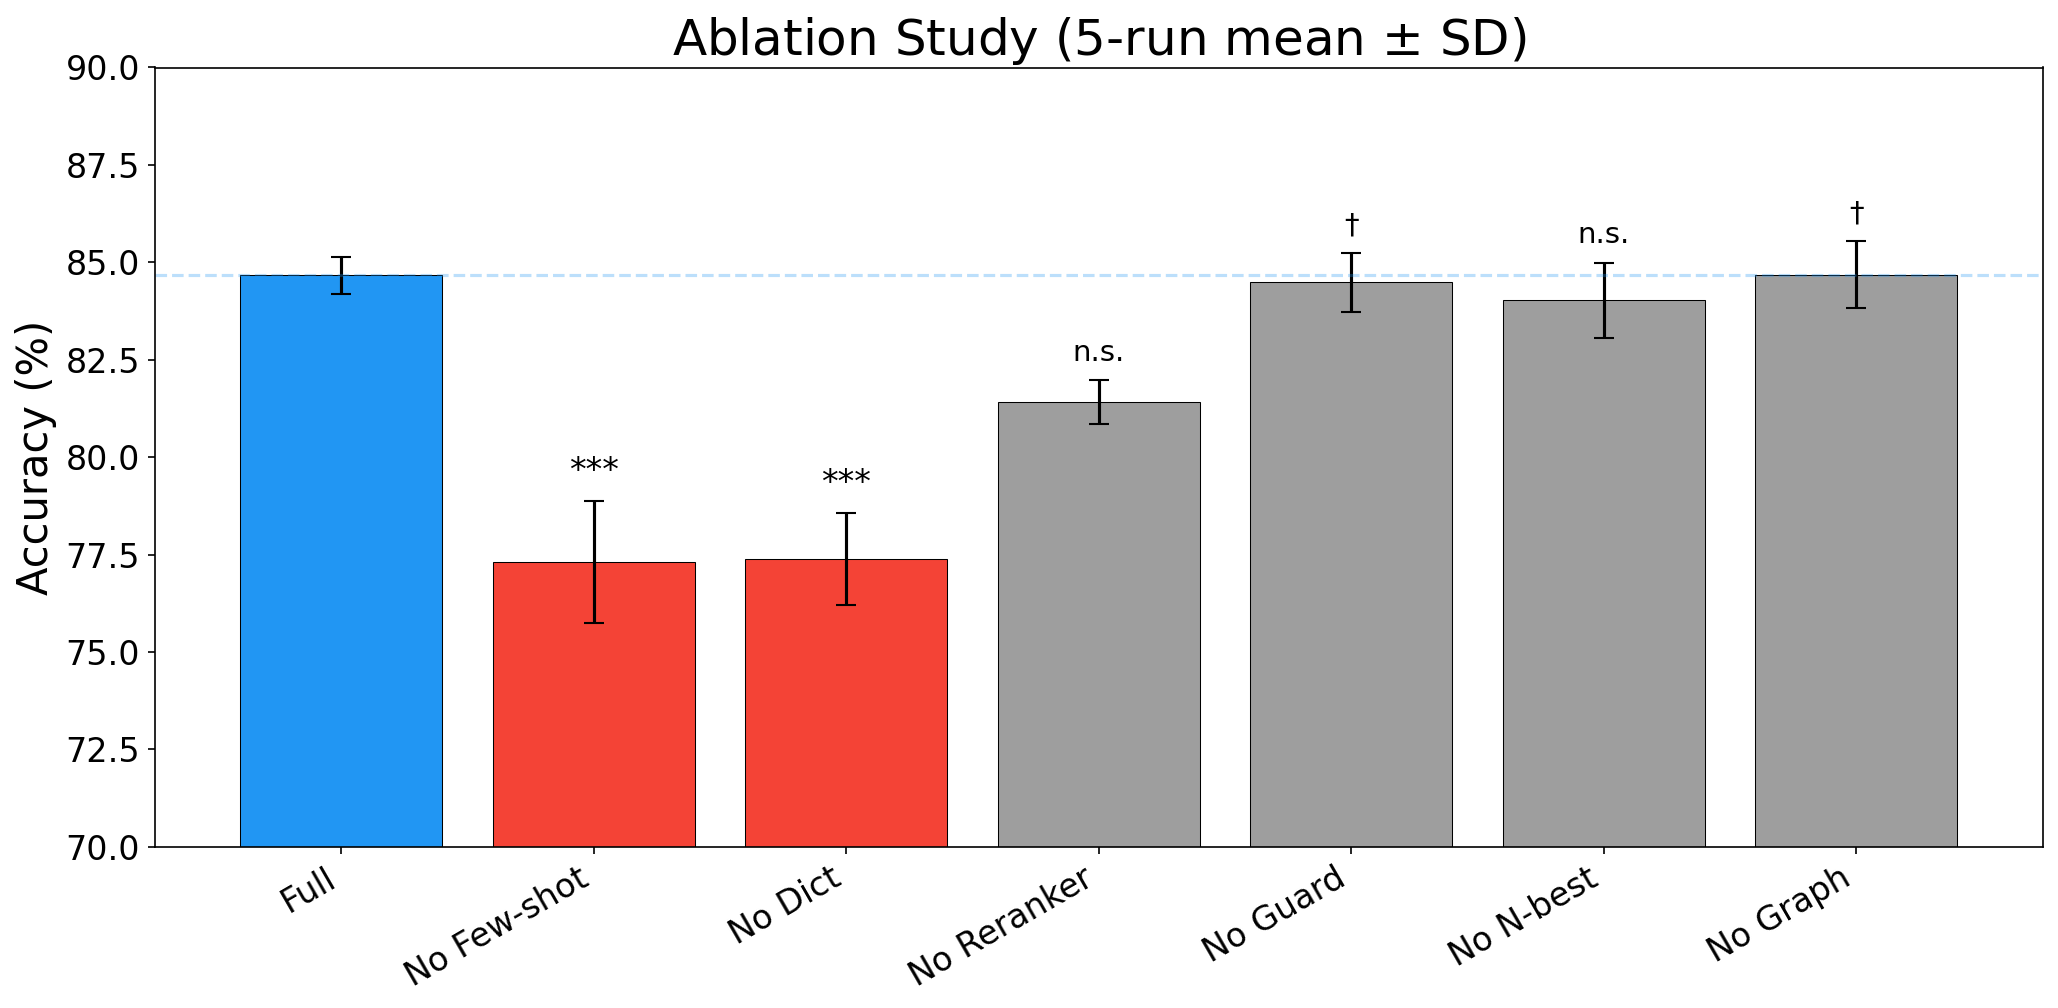
\includegraphics[width=\columnwidth]{figures/ablation_bar.png}
\caption{アブレーションスタディの棒グラフ（5回の平均 $\pm$ SD）。
赤い棒は統計的に有意な精度低下を示す条件を示す（$^{***}$: $p<0.001$）。星印の検定は表~\ref{tab:ablation}と同一の全符号置換検定（Wilcoxon符号順位統計量）のHolm補正後p値に基づく（no\_rerankerは補正後$p=0.0781$相当で有意でないためn.s.）。†は$n_\mathrm{nz}$が小さく検出力不足のため有意性判定を行わない条件（no\_guard・no\_nbest）を示す。}
\label{fig:ablation_bar}
\end{figure}

% =====================================================================

\subsection{LLM-onlyベースライン}
\label{sec:llm_only}

前節のアブレーションに加え、全構成要素を外した条件（LLM-only）を測定した。この条件では、\texttt{information\_schema}から機械的に列挙したスキーマ（テーブル・カラム・型の一覧とFKの組44件）、質問文、および主評価と同一の意味規約ノート（安定性の閾値、chemical\_systemの表記、統制語彙、site\_labelの規約）のみをGPT-5.5に与え、1回の呼び出しでSQLを生成させる。少数ショット例・辞書・スキーマリンク・FKグラフ制約・$n$-best・リランカー・SQLGuardは使用せず、後処理は応答からSQL部分を取り出す（コードフェンスの除去）だけである。生成SQLは同一DBで実行し、アブレーションと同一の期待結果で採点した。

\begin{table}[t]
\centering
\caption{LLM-onlyベースライン（GPT-5.5、245クエリ、単一ラン）。再現率・適合率・F1は行集合照合による平均（\%）。未解決参照・JOIN列は該当クエリ数（カラム：スキーマに解決できない修飾カラム名＝静的スキーマ未解決参照、JOIN：FK関係に基づかない結合）。未解決参照の計上はSQLテキストの静的照合（AST/エイリアス解決に基づくスキーマ許可リストとの突合）による診断であり、有効なCTE名や派生テーブル等の参照も計上し得るため、真の幻覚件数の上限的な診断値であって実行時エラー件数（実行成功率）とは一対一に対応しない。}
\label{tab:llm_only}
\footnotesize
\resizebox{\columnwidth}{!}{%
\begin{tabular}{@{}lrrrrrr@{}}
\toprule
難易度 & $n$ & 再現率 & 適合率 & F1 & \shortstack{未解決\\カラム参照} & JOIN幻覚 \\
\midrule
Easy      & 43  & 92.4 & 93.0 & 92.7 & 1  & 14 \\
Medium    & 69  & 82.6 & 88.0 & 83.4 & 20 & 29 \\
Hard      & 69  & 68.6 & 76.1 & 69.8 & 22 & 42 \\
VH        & 64  & 74.6 & 81.8 & 76.4 & 44 & 30 \\
\midrule
全体      & 245 & 78.3 & 83.9 & 79.4 & 87 & 115 \\
\bottomrule
\end{tabular}
}% end resizebox
\end{table}

結果を表~\ref{tab:llm_only}に示す。全体の実行再現率は78.3\%（適合率83.9\%、F1 79.4\%）であり、245クエリの主評価（セクション~\ref{sec:multiaxis}、再現率86.1\%）より7.8\,pp低い。この実行再現率は期待される行をどれだけ回収したかを測る行レベルの指標であり、生成SQLの出力が期待結果と完全に同一であった割合（厳密な完全結果集合一致10.6\%、セクション~\ref{sec:multiaxis}）とは別の指標である。構文の妥当性は100\%、実行成功率は99.6\%（VH層のみ98.4\%）であった。

誤った参照の発生率は種類によって異なる。スキーマに存在しないテーブルの参照は245クエリ中10件（クエリ内のテーブル参照に占める平均割合0.7\%）であった。一方、FK関係に基づかないJOINは115件（クエリ内のJOINに占める平均割合23.0\%）、スキーマに存在しないカラムの参照は87件（クエリ内のカラム参照に占める平均割合10.3\%、VH層では64件中44件）であった。これらの件数はSQLテキストを静的に照合して数えた診断値であり、有効なCTE名や派生テーブル由来の参照も含まれ得るため、実在しないスキーマ要素への参照件数の上限である。実行時エラーの件数とは一致しない。平均レイテンシは11.1秒であった。実行成功率は99.6\%であるのに対して再現率は78.3\%であり、誤りの大部分は実行エラーではなく、結合経路や列選択の誤りとして現れる。この種の誤りは実行時エラーの検出では見つけられない。

これらの誤りはパイプラインの各構成要素に対応する。FKに基づかないJOIN（115件）にはFKグラフによる結合経路の制約（セクション~\ref{sec:schema_graph}）、存在しないカラムの参照（87件）にはスキーマリンクとカラム許可リスト（セクション~\ref{sec:schema_link}）、Hard層の再現率低下には辞書と少数ショット例が対応する。主評価と比較すると、FKに基づかないJOINの割合は0.9\%から23.0\%へ、存在しないカラムの参照割合は4.0\%から10.3\%へ増加した。タスクは異なるが、汎用LLMの出力に材料ドメイン固有の誤りが残るという観察は、物性予測ベンチマーク~\cite{rubungo2025llmmatbench}の報告と一致する。

\subsection{感度分析}
\label{sec:sensitivity}

アブレーションで有意であった構成要素について、設定値を変えたときの感度を分析する。いずれもアブレーションと同一の手順・同一の100クエリサブセットによる単一ランである。したがって表~\ref{tab:ablation}のfull（5ラン平均92.5$\pm$0.4\%）とは直接比較できず、単一ラン間の小さな差はLLMの出力が毎回同一でないことによる変動の範囲内と解釈する（統計的な同等性は評価していない）。詳細な表と図は補足資料~\ref{sec:sup_results_details}に示す。

\subsubsection{少数ショット例の数の影響}
\label{sec:fewshot_sensitivity}

プロンプトに含める少数ショット例の数 $k$（セクション~\ref{sec:fewshot}の$k$）を1, 3, 5, 10, 15に変えた（表~\ref{tab:fewshot_k}、図~\ref{fig:fewshot_k}）。$k$を1から3に増やすと全体で$+$1.9\,pp（VH層で$+$10.0\,pp）上昇した。$k=3$（全体92.6\%、VH 88.4\%）と$k=15$（全体92.7\%、VH 88.4\%）はほぼ同等である（$k=5$：90.7\%、$k=10$：91.7\%）。レイテンシは$k$によらずほぼ一定（23.6--31.6\,s）であり、既定値は$k=3$とした。

\subsubsection{ドメイン辞書サイズの影響}
\label{sec:dict_sensitivity}

スキーマ写像辞書（61エントリ）と用語辞書を同時に、フル／50\%／25\%／10\%／0\%の5水準に削減して再評価した（表~\ref{tab:dict_size}、図~\ref{fig:dict_size}）。フルの91.8\%は表~\ref{tab:ablation}のfullとほぼ同水準であり、0\%の82.9\%とno\_dictの82.7\%はラン間の変動の範囲内で一致する。影響はVH層で最も大きく、フルから0\%への低下は$-$32.9\,pp（全体では$-$8.9\,pp）であった。Easy/Medium層は辞書の有無にかかわらずほぼ100\%／93--97\%である。辞書の効果は、専門用語をSQL条件へ変換する必要がある高難易度層に集中する。中間の水準（50\%・25\%・10\%）は86.0\%・85.0\%・85.0\%である。

\subsubsection{LLMモデルの影響}
\label{sec:model_comparison}

GPT-5.5とGPT-4oを比較した（表~\ref{tab:model_comp}、図~\ref{fig:model_comp}）。GPT-4oはレイテンシ2.1\,s（GPT-5.5の約1/15）で、全体の91.7\%はGPT-5.5のfullとほぼ同水準であった。層別ではMedium $-$3.4\,pp、Hard $+$5.0\,pp、VH $-$6.5\,ppであった。

% =====================================================================

\subsection{マルチ軸評価指標}

\label{sec:multiaxis}

主評価245クエリについて、実行再現率を補う複数の指標を計算した（層別の全指標は補足資料~\ref{sec:sup_results_details}の表~\ref{tab:multiaxis}・図~\ref{fig:radar}）。構文の妥当性と実行成功率は全層で100\%であった。この100\%は、SQLGuardによる検査と、実行に失敗する候補を選択段階で排除する$n$-best実行スコアリングの組み合わせによる結果であり、SQLGuardが任意の入力に対する安全性を保証することを意味しない。厳密な完全結果集合一致（ゴールドSQLの列リストと行の多重集合が一致し、\texttt{semantic\_ordered}契約が真の39クエリでは行順序まで一致）は10.6\%であった。一方、共通列への投影上でPrecision=Recall=1となる旧来の緩い完全一致は78.0\%（245クエリ、多軸評価と同一の単一ランに対する採点監査\texttt{scoring\_audit.json}の\texttt{common\_column\_exact\_overlap\_pct}；表~\ref{tab:scoring_audit}には列として掲載しない）であった。両者の差は、厳密な指標が列の追加や欠落に対して敏感であることを示す。実行再現率は86.1\%（適合率86.7\%、F1 85.3\%）、SELECT列精度（生成SQLが選択した列のうちゴールドSQLと一致した割合）は61.7\%であった。JOIN一致率（生成SQLのJOINがゴールドSQLと一致した割合）は全体で89.3\%、VH層で77.3\%であり、5つ以上のテーブルを結合するクエリでは貪欲最短経路連結による制約があってもJOIN経路の誤りが残る。スキーマに存在しないテーブル・カラムの参照割合はそれぞれ0.2\%・4.0\%、FKに基づかないJOINの割合は0.9\%であった。いずれもSQLテキストの静的な照合による診断値で、有効なCTE名や派生テーブル由来の参照も含まれ得る上限値であり、実行成功率100\%と矛盾しない。
\subsection{誤差分析}
\label{sec:error_analysis}

各アブレーション条件の誤り指標は補足資料~\ref{sec:sup_results_details}の表~\ref{tab:error_analysis}に示す。full条件では構文エラー、実行エラー、存在しないテーブルの参照はいずれも0件で、FK関係に基づかないJOINを含むクエリは5件であった（no\_graphで6件、no\_dictで4件、no\_nbestでは実行エラー3件）。no\_nbestでのみ実行エラーが残ることは、実行に失敗する候補を選択段階で排除する機構が働いていることを示す。

保存されたfull条件のラン（245クエリの多軸評価ラン）で再現率が0.8未満だったのは39件（VH 17・Hard 15・Medium 5・Easy 2）であった。誤りの種類を機械的に分類する（1件に複数の種類が付き得る）と、誤ったカラム選択（SELECT列精度0.5未満：24件）と、ゴールドSQLが参照するテーブルの一部欠落（JOIN不一致：24件）が主な要因で、GROUP BYの欠如（14件）、値の不一致（4件）が続く（図~\ref{fig:error_dist}；母集合と定義は補足資料~\ref{sec:sup_results_details}）。今後の改善対象は、導出量や複合スコアの定義を含むSELECT句の生成である。

% =====================================================================

\subsection{SQLインジェクションと安全性}

\label{sec:injection_safety}

7つの悪意ある入力でSQLGuardを検証した（セクション~\ref{sec:sqlguard}）。内訳は、DROP/DELETE/INSERTなどデータを破壊する操作を自然言語の質問文に混ぜた5件（テストID E01--E05）と、SQL文をそのまま入力した2件（同F01--F02）である（各ケースの入力と判定は表~\ref{tab:injection_results}）。
E01--E05は禁止キーワードの検出、複数文の検出、テーブル許可リストなどで棄却された。F01はSELECT文の直接入力であり、LIMITが自動追加されて実行される（棄却されない）。F02はDMLの検出で棄却される。これら7ケースは同梱の検証スクリプトで再検証できる。no\_guard条件での実行再現率の変化は$-$0.2\,pp（検出力不足のため有意性は判定しない）であり、この安全層の目的は再現率の向上ではなく、危険なSQLを実行前に排除することである。

% =====================================================================

\subsection{材料工学評価}
\label{sec:materials_evaluation}

材料研究で実際に行われる問い合わせの例として、次の3つの探索を検証RDB上で実行した。(1) $\gamma'$相候補のランキング：安定性・格子定数の一致・体積弾性率の3指標を重み付けした複合スコアで、255の異なるL1$_2$組成を順位付けした（157の安定/準安定候補のうちNi$_3$Alが1位）。(2) Ni$_3$Alに近い格子定数を持つ候補の抽出：$|a - a_{\text{Ni}_3\text{Al}}| \leq 0.03$~\AA{}{}（$a_{\text{ref}} = 3.572$~\AA{}{}）を満たす26の組成（27エントリ）を抽出した（全27エントリは補足資料の表~\ref{tab:lattice_match}）。(3) 安定/準安定候補の抽出：$E_\text{hull} \leq 0.05$~eV/atomの157件（安定7件（$E_\text{hull} \leq 0.001$）、準安定150件）を抽出した。表~\ref{tab:gamma_prime}（全10行は補足資料の表~\ref{tab:gamma_prime_full}）と表~\ref{tab:lattice_match}の数値は、数値集約スクリプトが検証済みのSQL（ゴールドSQLと同型の決定的なSQL）をDBに対して実行した結果であり、パイプラインが生成したSQLの出力そのものではない（同型の質問はパイプライン評価では成功と失敗の双方がある；補足資料~\ref{sec:sup_query_detail}）。化合物の属性値は合成検証データであるため、これらの結果を実材料の設計仮説として解釈してはならない。

$\gamma'$相候補ランキングは組成（formula）単位で複合スコア
\begin{equation}
  S = w_1 \cdot S_\text{stability} + w_2 \cdot S_\text{lattice} + w_3 \cdot S_\text{bulk}
  \label{eq:composite_score}
\end{equation}
により行った（$w_1 = 0.35$、$w_2 = 0.35$、$w_3 = 0.30$；$S_\text{stability} = 1 - E_\text{hull}/0.05$、$S_\text{lattice} = 1 - |\Delta a|/0.3$、$S_\text{bulk} = B/300$；同一組成に複数のエントリがある場合は$S$が最大のもので代表させる）。Ni$_3$Alは低い$E_\text{hull}$と小さい$\Delta a$により1位、既知の安定L1$_2$相であるCo$_3$Ti（$\Delta a = 0.022$~\AA{}{}、$E_\text{hull} = 0.0$）が2位であり、Co$_3$Tiは格子定数候補の抽出結果にも含まれる。Cr$_3$InやPt$_3$Tiのようなエントリが上位に現れるのは、合成データセットが大きな体積弾性率を割り当てているためである。安定7相のうち生成エネルギーが最も低いのはPt$_3$Al（$E_f = -0.550$~eV/atom）で、Al$_3$Sc（$-0.500$）、Co$_3$Ti（$-0.450$）、Cr$_3$Fe（$-0.440$）、Ni$_3$Al（$-0.420$）が続く。

\begin{table}[t]
  \centering
  \caption{$\gamma'$-相候補ランキングの上位5行（複合スコア$S$；全10行と\texttt{entry\_id}・$a$・$B$は補足資料の表~\ref{tab:gamma_prime_full}）。化合物属性は合成検証データである。}
  \label{tab:gamma_prime}
  \footnotesize
  \begin{tabular}{rlccc}
    \toprule
    ランク & 化合物 & $E_\text{hull}$ & $\Delta a$ (\AA{}{}) & $S$ \\
    \midrule
    1 & Ni$_3$Al & 0.000 & 0.000 & 0.880 \\
    2 & Co$_3$Ti & 0.000 & 0.022 & 0.864 \\
    3 & Cr$_3$In & 0.012 & 0.025 & 0.839 \\
    4 & Hf$_3$V & 0.006 & 0.018 & 0.834 \\
    5 & Pt$_3$Sc & 0.003 & 0.035 & 0.833 \\
    \bottomrule
  \end{tabular}
\end{table}

% =====================================================================

\section{考察}
\label{sec:discussion}

\subsection{スキーマ理解の障壁と自然言語アクセス}

アブレーションの結果は、無機材料RDBを利用する際の主な障壁がSQLの文法ではなく、正規化スキーマの構造と結合経路の理解にあることを示す。no\_fewshot（76.4\%）とno\_dict（82.7\%）はfull（92.5\%）を下回り（表~\ref{tab:ablation}）、VH層ではそれぞれ65.7\%、52.0\%に低下する。低下は専門用語を多く含む複雑なクエリに集中する。構文の妥当性と実行成功率が100\%（表~\ref{tab:multiaxis}）、JOIN一致率が89.3\%であることは、生成SQLが実行可能でFK関係に沿っていることを示す。スキーマの変更については、FKメタデータに基づく設計のためテーブルの追加やFKの変更は自動的に反映され、辞書と少数ショット例の更新は定型的な手順で行える。

\subsection{コンポーネント別の寄与}
\label{sec:reranker_discussion}

\paragraph*{少数ショット例}
少数ショット例を外したときの低下が最も大きかった（$-$16.1\,pp, $p<0.001$；Hard層$-$24.7\,pp、VH層$-$21.8\,pp、Medium層$-$12.7\,pp；表~\ref{tab:ablation-detail}）。Hard/VH層の低下は、スキーマの全文と辞書を与えても、LLMだけでは多テーブルの結合や多段の集約を含むSQLを組み立てにくいことを示す。

\paragraph*{材料ドメイン辞書}
辞書を外すと全体で$-$9.8\,pp低下した（$p=0.0001$、Holm補正後も有意）。効果は難易度層によって異なり、Easy層では低下がなく、Medium層は$-$1.3\,ppにとどまる一方、Hard層は$-$7.7\,pp、VH層は$-$35.5\,ppであった（表~\ref{tab:ablation-detail}）。Easy/Mediumのクエリは一般的な表現で構成されており、LLMがSQL条件を推測できる。これに対してVHのクエリは複数の専門用語（例：``$\gamma'$相'' $\to$ \texttt{structure.prototype = 'L12'}）を同時に含み、辞書なしでは正しい条件を生成しにくい。辞書は同義語・別名・表記の揺れをSQL条件へ統一的に変換する語彙資源であり、SQLの書き方を示す少数ショット例とは役割が異なる。

\paragraph*{リランカー}
リランカーを外すと$-$6.2\,pp低下した（未補正$p=0.0195$だがHolm補正後$p=0.0781$で有意ではない）。効果はMedium層（$-$13.0\,pp）・Hard層（$-$6.5\,pp）に集中した（表~\ref{tab:ablation-detail}）。別途実施したリランカー単独の比較評価（20クエリ、有無の両条件を同一条件で再生成した単一ラン）では、あり92.2\%、なし77.7\%（$+$14.5\,pp；差は未丸め値から算出）であった。

\paragraph*{SQLGuard・$n$-best・貪欲最短経路連結}
SQLGuard（$-$0.2\,pp、95\%CI $[-0.6, +0.1]$\,pp）、$n$-best（$-$0.3\,pp、$p=0.625$、95\%CI $[-1.1, +0.4]$\,pp）、貪欲最短経路連結（$-$1.4\,pp、$p=0.1484$、95\%CI $[-3.4, -0.002]$\,pp）は、いずれも実行再現率に有意な効果を示さなかった。SQLGuardと$n$-bestは非同点ペアがそれぞれ2・5件と少なく、検定の検出力が不足するため有意性の判定を行っていない（表~\ref{tab:ablation}の†）。これは効果がないことや同等であることの証拠ではない。SQLGuardの役割はSQLインジェクションやSELECT以外の文を実行前に排除することである（構文妥当率100\%はSQLGuard単独の効果とは解釈しない）。$n$-best = 1は精度をほぼ維持しつつ、レイテンシを30.9\,sから8.6\,sに短縮する（表~\ref{tab:latency}）。

貪欲最短経路連結を外しても有意な差はなかった。FKに基づかないJOINを含むクエリは、この保存ランではfullで5件、no\_graphで6件と少ない（表~\ref{tab:error_analysis}）。この構成要素の役割は、JOINをFK関係に沿って構成することにある。全体精度に差が出ない一因は、本検証DBが36テーブルであり、スキーマの全文がプロンプトに収まる規模であることである。これは、スキーマリンクの精度への寄与が大規模なスキーマで現れるという先行研究の観測~\cite{maamari2024schema}と一致する。no\_graphの$-$1.4\,pp（有意でない）はスキーマ規模に依存した観測であり、より大規模な正規化RDB（Materials Project~\cite{jain2013mp}、AFLOW~\cite{curtarolo2012aflow}）での効果は未検証である。

\paragraph*{寄与の相互作用}
アブレーションは構成要素を1つずつ外す方式であり、要素間に相互作用があるため、各要素の寄与を足し合わせても全体の効果にはならない。同一DB上での他手法（DIN-SQL、DAIL-SQL等）との直接比較は行っていない（制限事項参照）。LLMのみ／スキーマのみの構成で生成されたSQLの例は補足資料~\ref{sec:sup_sql_examples}に示す。

\subsection{追加検証：独立設計クエリ・多段計算・一般化・言語}
\label{sec:additional_validation}

主評価（245クエリ；うち100クエリは共同著者による独立設計）とアブレーションは、著者らが設計したクエリと単一のDBに閉じている。本節では(1)~独立設計100クエリの別ラン再評価、(2)~CTEを要する多段計算クエリ、(3)~列間比較クエリ、(4)~適応条件の異なる4種の一般化試験、(5)~質問文の言語への依存性、を報告する。このうち独立設計100クエリ・バリアントA 20クエリ・CTE 15クエリは、主評価245クエリの部分集合（表~\ref{tab:main_partition}；計135クエリ）を別のランで再評価したものであり、245クエリの外に追加した評価コーパスではない。一方、一般化バリアントB/C/D（計55クエリ）と非翻訳英語25クエリは、主評価に含まれない別のコーパスである。

\subsubsection{独立に設計されたクエリによる評価}
\label{sec:independent_eval}

辞書と少数ショット例を設計した著者が評価クエリも作成すると、クエリがパイプラインの得意なパターンに偏り、精度を過大に評価する可能性がある（自己参照バイアス）。このため主評価245クエリ（セクション~\ref{sec:query_design}）には、実装に関与していない共同著者が独立に設計した100クエリを含めた（表~\ref{tab:main_partition}）。本項ではこの100クエリだけを別のランで再評価した結果を報告する。難易度分布はEasy 18 / Medium 34 / Hard 34 / Very Hard 14で、基本検索から材料設計・統計まで10カテゴリにわたる（内訳は補足資料~\ref{sec:sup_expert_queries}）。採点はアブレーションと同じ実行再現率と難易度分類で行った。

この別ランの全体実行再現率は81.5\%（Easy 87.8\% / Medium 90.5\% / Hard 70.2\% / Very Hard 78.7\%；平均レイテンシ29.9\,s）であった。この100クエリは主評価245クエリに含まれるため、主評価全体（86.1\%）との単純な差4.6\,ppを、著者設計と独立設計の差と解釈することはできない。主評価の単一ラン内では、同じ独立設計100クエリの部分が83.4\%、残りの著者設計145クエリが87.9\%であり、主評価全体との差には同一100クエリのラン間変動（83.4\% 対 81.5\%）も混ざる。自己参照バイアスの定量値としては、同一ラン内での部分集合の比較（独立設計83.4\% 対 著者設計87.9\%、4.5\,pp）が適切である。ただしこれも、問題分布の差を含む探索的な観察である。この差が難易度分布の違い（著者設計145クエリはVHの比率が高い：50/145 対 14/100）による見かけ上のものでないかを確認するため、両部分集合の層別実行再現率を主評価コーパス全体の難易度構成（43/69/69/64）に合わせて標準化すると、独立設計83.9\% 対 著者設計89.4\%（5.5\,pp）と差は広がる（層別ではEasy 87.8\% 対 100.0\%、Medium 90.5\% 対 97.1\%、Hard 73.2\% 対 88.6\%、VH 85.7\% 対 74.8\%で、VHのみ逆転）。したがって難易度構成比の違いだけではこの差は説明できない。ただし、同一層内での構造的な複雑さ（SQL長・テーブル数・サブクエリ数）や少数ショット例の被覆度は統制していないため、この標準化比較も探索的な観察である。独立設計クエリの値が低い要因の候補は、(1)~\texttt{elastic\_tensor}や\texttt{magnetic\_property}など、少数ショット例が少ない周辺テーブルの参照、(2)~著者設計クエリの決まったパターン（「L1$_2$」の明示）に合わせて作られた少数ショット例、(3)~条件を暗黙に指定する表現を含む語彙の多様性、である。ただし周辺テーブルの参照だけでは説明できない。非翻訳英語25問（セクション~\ref{sec:language_eval}）も\texttt{magnetic\_property}や\texttt{surface\_energy}などを参照するが$96.5$\%であり、両データセットは構造的な複雑さが異なる。

構文の妥当性（100.0\%）は両セットで一致する。VH層（78.7\%）がHard層（70.2\%）より高いのは、VHクエリの多くが少数ショット例に含まれる短いCTEパターンを含むのに対し、一部のHardクエリは例のない周辺テーブルを参照するためである（詳細は補足資料~\ref{sec:sup_expert_queries}）。

\subsubsection{多段階計算クエリとCTE評価}
\label{sec:multistep_query}
\label{sec:cte_eval}

材料研究の問いには、複数の物理量から別の量を計算する多段階のクエリが含まれる。代表例``Ni$_3$Alの生成エンタルピーを純元素参照を用いて計算せよ''では、3テーブルからデータを取得し、$\Delta H_\mathrm{f} = E_\mathrm{total} - \sum_i x_i E_\mathrm{ref}(i)$（$E_\mathrm{total}$は化合物の全エネルギー、$E_\mathrm{ref}$は純元素の参照エネルギー、$x_i$は元素$i$の組成比）を計算するCTEへ変換する必要がある。本パイプラインは、\texttt{formation\_enthalpy}ビューを通じた単純なクエリと、少数ショット例に基づく明示的なCTE計算の両方に対応する。従来のベンチマーク（Spider~\cite{yu2018spider}、BIRD~\cite{li2024bird}）はこうした導出量の計算を含まない。

CTEを要するクエリをアブレーション条件ごとに評価した（カテゴリ構成と結果表は補足資料~\ref{sec:sup_discussion_details}、表~\ref{tab:cte_results}）。few-shot例に含まれる既知の5パターンはfull条件で100.0\%であり、少数ショット例を外すと60.0\%、辞書を外すと80.0\%に低下した。一方、リランカー・SQLGuard・グラフJOIN制約を外しても100\%を維持した（$n$-bestを外すと96.0\%）。さらに、主評価245クエリに含まれるCTEクエリ15件（アブレーション用サブセット内の既知5パターンと、245クエリに含まれるがアブレーション対象外の10クエリ。後者はウィンドウ関数、2段階の集約、3段階のCTEなど、少数ショット例に含まれないゼロショットのパターン）を別のランで評価した。既知の5パターンは100\%を維持したが、ゼロショットの10パターンは59.0\%であった（全体72.7\%）。多段計算に対応できる範囲は少数ショット例のパターンの範囲で定まり、新しいパターンへの対応は例の追加で行う。

\subsubsection{列間比較クエリの取り扱い}
\label{sec:column_comparison}

「値Aが値Bより小さいエントリ」のように同じ行の中で2つの列を比較する条件（\texttt{WHERE col\_a > col\_b}）は材料研究でよく現れる。この条件は定数との比較（\texttt{WHERE col > 0.5}）に比べてLLMが正しく生成しにくく、異なるテーブルの列を比較する場合は各列がどのテーブルに属するかを特定する必要がある。本パイプラインは、同一テーブル内の比較、テーブル間の比較、集約関数を用いた比較の3種類を少数ショット例として供給する（例プールは主にこのパターンで45例に拡張した；SQL断片は補足資料~\ref{sec:sup_column_comparison}）。

\subsubsection{異なる適応条件における一般化評価}
\label{sec:transfer_eval}

適応条件の異なる4種の一般化試験を実施した（表~\ref{tab:transfer_eval}）。Aは同一の36テーブルスキーマのまま、対象プロトタイプをL1$_2$以外に広げる試験であり、スキーマの変更は含まない。BとCはパイプラインのコードを変更せずに別のスキーマへ適用するが、転送用のプロンプトテンプレートを用いる。Dはコード変更なしであるが、Materials Project（MP）スキーマ用のプロンプトと8件のMP専用few-shot例を与える軽量なスキーマ適応である。したがって、4条件をまとめて「適応なし」とは呼ばない。表の百分率は実行再現率である。

\begin{table}[t]
\centering
\caption{一般化評価の結果。百分率は行レベルの実行再現率であり、適応条件はバリアントごとに異なる。Aの20クエリ（\texttt{q\_proto\_*}）は主評価245クエリの部分集合であり、100.0\%は同一問題に対する別ランの値である（主評価の単一ラン内では同20クエリは85.0\%であり、差はラン間変動を含む）；B/C/Dは主評価に含まれない別コーパスである。}
\label{tab:transfer_eval}
\footnotesize
\begin{tabular}{@{}lp{11.5em}cc@{}}
\toprule
バリアント & スキーマ／適応条件 & $n$ & 再現率 \\ \midrule
A & 同一スキーマ・5プロトタイプ横断クエリ & 20 & 100.0\% \\
B & OQMD風リネーム（コード変更なし） & 20 & 85.0\% \\
C & 識別子難読化（コード変更なし） & 20 & 80.0\% \\
D & MP実データ（MP専用prompt + few-shot） & 15 & 93.3\% \\
\bottomrule
\end{tabular}
\end{table}

Dの結果はスキーマに依存しないことの証明ではなく、軽量な適応を行った結果である。条件カテゴリとテーブル名の対応表など、元のスキーマを前提とする要素が残るため、スキーマ非依存とは主張しない（各バリアントの詳細と解釈上の注意は補足資料~\ref{sec:sup_discussion_details}）。

\subsubsection{言語依存性の検証}
\label{sec:language_eval}

質問文の言語への依存性を2種類の評価で検証した。第一に、アブレーションで用いた100クエリの質問文を意味の等しい英語に翻訳し、gold SQL・期待結果・データベース・パイプライン構成を固定したまま質問文の言語だけを変える対応あり比較（paired比較）を行った（full条件、各言語3ラン）。行レベル実行再現率は日本語$92.0 \pm 0.7$\%（3ラン：91.8／91.4／92.7\%）、英語は日本語より平均$2.0$\,pp低かった（$90.0 \pm 2.0$\%、3ラン：91.7／90.4／87.8\%；表~\ref{tab:language_eval}）。日本語の$92.0$\%は表~\ref{tab:ablation}のfull条件$92.5 \pm 0.4$\%（5ラン）とは別の3ランであり、両者はラン間変動の範囲で整合する\footnote{層別ではpaired日本語（3ラン）はHard 88.9\%・Very Hard 81.9\%で、表~\ref{tab:ablation}のfull（5ラン）のHard 86.8\%・Very Hard 87.5\%と差があるが、クエリ単位で照合するとこの層別差は主として2クエリ（q\_hard\_014：$0.00 \to 0.67$、q\_vhard\_005：$1.00 \to 0.00$）のラン間変動に由来し、層ごとの$n$が小さい（Hard 30・Very Hard 20）ための見かけの差である。}。クエリ単位の3ラン平均に対する対応あり検定では、Wilcoxon符号順位統計量に対する全符号置換検定（差が0でない13件について$2^{13}$通りの符号の割り当てをすべて列挙して分布を求める方法；同順位は中央順位で処理）で$p=0.193$、平均差のブートストラップ95\%信頼区間は$[-5.8, +1.6]$\,ppで0を含み、言語による差は検出されなかった。ただしこれは、両言語が同等であることや、言語一般に依存しないことの証明ではない。未丸めのクエリ単位3ラン平均に基づく層別差（EN$-$JA）はEasy $-1.3$\,pp（非同点2件）、Medium $-3.3$\,pp（非同点2件）、Hard $+0.2$\,pp（非同点6件）、Very Hard $-4.1$\,pp（非同点3件）であるが、非同点ペア数が少ないため探索的な観測にとどまる（表~\ref{tab:language_eval}はラン単位平均の層別値であり、その表示値の差とはここでの丸め・集計順序の違いにより最大$0.1$\,pp程度ずれる）。なお、paired評価ではfew-shot例プール（45例、質問文はすべて日本語）を英語用に差し替えず日本語のまま固定した。本評価は日本語と英語の2言語に限られ、言語一般に対する非依存性を示すものではない。

\begin{table}[t]
\centering
\caption{言語依存性検証（paired比較）の結果。100クエリ・full条件・各言語3ランの行レベル実行再現率（3ラン平均、\%）。gold SQL・期待結果・データベース・パイプライン構成は両言語で同一。}
\label{tab:language_eval}
\footnotesize
\resizebox{\columnwidth}{!}{%
\begin{tabular}{@{}lccccc@{}}
\toprule
言語 & 全体（mean $\pm$ SD） & Easy & Medium & Hard & Very Hard \\ \midrule
日本語 & $92.0 \pm 0.7$ & 99.7 & 96.7 & 88.9 & 81.9 \\
英語 & $90.0 \pm 2.0$ & 98.3 & 93.3 & 89.1 & 77.8 \\
\bottomrule
\end{tabular}
}% end resizebox
\end{table}

第二に、既存の評価セットを参照せずに英語で新たに25問を作成し、作問後にgold SQLと期待結果を作成してデータベース上で検証したうえで、同一のパイプライン・同一の採点で評価した（3ラン）。難易度ラベルはgold SQLからセクション~\ref{sec:query_design}の設計時難易度層のpost-hoc複雑さ指標で機械的に算出し（再現パッケージの\texttt{compute\_unified\_difficulty.py}。同スクリプトは設計時の構造的複雑さ基準を再現可能に近似する事後指標の実装であり、著者が設計時に付与した主評価245問の既存ラベルとは144/245で一致、不一致101件のうち92件（91.1\%）は隣接層間のずれである）、Easy 13・Medium 8・Hard 4・Very Hard 0である。実行再現率は$96.5 \pm 2.3$\%（95.2／95.2／99.2\%）であった。ただし、この25問は難易度分布が主評価と異なり（Very Hardを含まず、テーブル数・CTE・SQL長などの構造的複雑さも主評価のHard／Very Hard層より低い）、$96.5$\%を主評価86.1\%やpaired日本語92.0\%と直接比較することはできない。この評価は翻訳を経ない英語クエリに対する補助的な確認である。なお、この25問には\texttt{expected\_tables}等の多軸メタデータを付与しておらず、多軸指標（SELECT列精度・JOIN一致率等）は算出していない。両評価のデータセット・gold SQL・期待結果・評価スクリプト・実行ログは再現パッケージに含まれる。

\subsection{RDBスキーマ設計とText-to-SQLコスト}
\label{sec:schema_design_cost}

正規化されたスキーマでは1つの質問に複数のJOINが必要となり、生成すべきSQLが複雑になる。本データベースの生成エンタルピー計算（セクション~\ref{sec:multistep_query}）は\texttt{phase\_stability}・\texttt{composition}・\texttt{pure\_element\_reference}の3テーブルのJOINとCTEによる集約を要する。少数ショット例なしでの$-$16.1\,ppの低下は、結合のパターンが複雑になるほどSQL生成が難しくなることを示す。Text-to-SQLでの利用を前提とするなら、DB側で次の設計が取れる。(1) 多段階のJOINをビュー（本研究の\texttt{formation\_enthalpy}ビューがその例）にまとめ、単一のSELECTで問い合わせられるようにする。(2) 頻繁に参照されるテーブル群（例：\texttt{composition}と\texttt{element}）をあらかじめ結合して非正規化する。(3) 列名にテーブルの文脈を含める（\texttt{energy} $\to$ \texttt{formation\_energy\_per\_atom}）。(4) FK制約を明示的に定義する。(4)は、本実装の貪欲最短経路連結がFK関係のみからJOIN経路を構成するため必須である。OQMD、Materials Project、AFLOWなどの無機材料RDBは正規化スキーマとFKメタデータを持つため、本パイプラインはFK情報の読み取りと辞書・少数ショット例の差し替えで適応できる（一般化試験D、セクション~\ref{sec:transfer_eval}）。DB側が上記の設計を採れば、Text-to-SQL側で辞書と例を整備するコストは下がる。

\subsection{類似無機材料RDBへの拡張性}
\label{sec:extensibility}

FK情報の読み取りに基づく貪欲最短経路連結は、FK制約が明示されたRDBであればグラフを自動構築できる。辞書の4カテゴリ構造（プロトタイプの別名、元素名の対応、安定性用語、物性用語）は無機材料RDB一般に適用できる。ただし、必要テーブルの意味付けや条件カテゴリとテーブルの対応にはスキーマ固有の情報が残り、少数ショット例は検証DBのスキーマに依存するため、別のRDBへ適用する際には例を設計し直す必要がある。異なる意味論を持つRDBや大規模なRDBへの一般化性能は主張しない。

\subsection{関連システムとの比較}

既存のText-to-SQL手法は一般分野向けであり、材料科学の正規化RDBを対象としていない。材料分野の自然言語アクセス手法はAPIやRDF/SPARQLを用いており、既存のRDBに対するSQL生成には対応しない。本研究は、正規化RDB・材料分野の知識・FKグラフ探索の組み合わせを対象とする（表~\ref{tab:related_comparison}）。

\begin{table*}[htbp]
  \centering
  \caption{関連する材料NLP / T2SQL / オントロジーシステムとの比較。}
  \label{tab:related_comparison}
  \footnotesize
  \begin{tabularx}{\textwidth}{llccccX}
    \toprule
    タイプ & 名前 & \shortstack{スキーマ\\対応} & \shortstack{正規化\\RDB} & \shortstack{材料\\特有} & \shortstack{NL$\to$\\クエリ} & 主な違い \\
    \midrule
    \multicolumn{7}{l}{\textit{T2SQLベンチマーク}} \\
    データセット & Spider~\cite{yu2018spider} & はい & はい & いいえ & SQL & 一般的なベンチマーク \\
    データセット & BIRD~\cite{li2024bird} & はい & はい & いいえ & SQL & 大規模な実データ \\
    \midrule
    \multicolumn{7}{l}{\textit{T2SQL手法}} \\
    手法 & DAIL-SQL~\cite{gao2023dail} & はい & はい & いいえ & SQL & スケルトン選択 \\
    手法 & RAT-SQL~\cite{wang2020ratsql} & はい & はい & いいえ & SQL & 関係認識エンコーディング \\
    手法 & RESDSQL~\cite{li2023resdsql} & はい & はい & いいえ & SQL & スキーマリンク分離 \\
    手法 & SchemaGraphSQL~\cite{safdarian2026schemagraphsql} & はい & はい & いいえ & SQL & パス探索 \\
    \midrule
    \multicolumn{7}{l}{\textit{材料情報学}} \\
    手法 & MKNA~\cite{zhuang2026mkna} & いいえ & いいえ & はい & API & エージェント \\
    手法 & OptiMat~\cite{hu2026optimat} & いいえ & いいえ & はい & API & オンデマンドDFT \\
    \midrule
    \multicolumn{7}{l}{\textit{オントロジー}} \\
    手法 & SuperCon~\cite{ishii2023supercon} & はい & いいえ & はい & SPARQL & RDFオントロジー \\
    手法 & PoLyInfo~\cite{ishii2024polyinfo} & はい & いいえ & はい & SPARQL & BFO準拠 \\
    \midrule
    手法 & 提案手法 & はい & はい & はい & SQL & FKトラバーサル + 材料辞書 \\
    \bottomrule
  \end{tabularx}
\end{table*}


最も近いSchemaGraphSQL~\cite{safdarian2026schemagraphsql}との違いは次の3点である。(1)~材料ドメイン辞書による用語の変換（外すと$-$9.8\,pp, $p=0.0001$）を備える。(2)~JOIN経路の探索がエッジ重みの最適化ではなく、FKグラフ上の貪欲最短経路連結（最小性は保証しない）である。(3)~ASTに基づくSQL安全性検証（SQLGuard）を含む。

\subsection{制限事項と今後の研究}

主な制限は以下の10点である。
\begin{enumerate}[nosep]
  \item 単一データベースでの検証：主評価はL1$_2$を中心に5プロトタイプを含む検証DB（36テーブル、1ビュー、1{,}559エントリ、全テーブル総行数21{,}703行（約2.2万行））に基づく。格納データのうちOQMDのDFT計算値をそのまま用いたのは純元素の参照エネルギー（\texttt{pure\_element\_reference}、2参照セット$\times$89元素＝178行）のみで、他は合成検証データである。一般化評価（セクション~\ref{sec:transfer_eval}）は条件が同一ではなく、異なる意味論や規模を持つRDBへ無修正で一般化できることは確認していない。
  \item 36テーブル・1ビュー構成の限界：スキーマの規模は実際の材料RDBより小さく、属性名の多様さ（同義語、略語、複数言語）や異なる正規化方針を網羅していない。スキーマのメタデータだけでは解決できない暗黙の知識（例：特定の材料系における「安定」の意味）も残る。
  \item 統計検定の範囲：検定では各クエリの5ラン平均実行再現率をクエリの値とし（$n=100$）、full条件と各除去条件の対応あり差に対して、Wilcoxon符号順位統計量の全符号置換検定（同順位は中央順位で処理；差が0のペアは除外し、非同点ペア数$n_\mathrm{nz}$を併記。セクション~\ref{sec:language_eval}の言語比較と同一の検定）を行った。全体の$\Delta$にはクエリ単位のブートストラップ95\%CIを付与した（表~\ref{tab:ablation}）。no\_guard（$n_\mathrm{nz}=2$）・no\_nbest（$n_\mathrm{nz}=5$）は非同点ペアが少なく、検定の検出力が不足する。5回の反復では層別（特にVH、$n=20$）の信頼区間を評価するには不十分であり、層別の$\Delta$は探索的な分析にとどまる。
  \item クエリのカバレッジ：主評価245クエリ（著者設計145＋共同著者による独立設計100）は実使用の多様なパターンを網羅しない。
  \item 難易度スコアの妥当性：スコアはゴールドSQLの構造的な複雑さを測るもので、LLMにとっての実際の難しさとは必ずしも単調に対応しない（独立設計ではVH 78.7\% $>$ Hard 70.2\%。LLM-onlyベースラインでも同じ傾向のVH 74.6\% $>$ Hard 68.6\%が観測され、この非単調性はパイプライン固有ではない）。これは、few-shot例が一部のVHパターン（短いCTEなど）を含む一方で、few-shot例に対応するものがないHardクエリが存在するためである。few-shot例の被覆度を加味した指標は今後の課題である。
  \item 辞書の収載範囲：492用語の辞書はL1$_2$系の探索に特化しており、他の材料系への拡張には手動での登録が必要である。表記の揺れの吸収（例：\texttt{prototype}／\texttt{strukturbericht}両カラムへのOR展開）は辞書に登録済みの別名にのみ保証され、未登録の同義語・略記は検索漏れとなり得る。
  \item あいまいな自然言語表現：「安定な」などの語の解釈はユーザーによって異なり得る（本評価ではセクション~\ref{sec:query_design}の定義に固定した）。問いを具体化する対話インターフェースを併用する余地がある（具体例は補足資料~\ref{sec:sup_ambiguous}）。
  \item 使用言語への依存性：主評価のクエリは日本語である。セクション~\ref{sec:language_eval}のpaired比較では英語でも$90.0 \pm 2.0$\%（日本語$92.0 \pm 0.7$\%、日本語比$-2.0$\,pp）であり、対応あり検定では差は検出されなかった（Wilcoxon符号順位統計量の全符号置換検定$p=0.193$、95\%CIは0を含む）。層別のMedium（$-3.3$\,pp）・Very Hard（$-4.1$\,pp）の低下は非同点ペアが各2・3件の探索的な観測である。日本語の比較表現向けパーサ、日本語のfew-shot例、日英辞書の英語側の整備状況は、依存要因の候補にとどまる（本データは依存を証明しない）。翻訳を用いない英語25問でも$96.5 \pm 2.3$\%であったが、難易度分布が主評価と異なるため水準の直接比較はできない。日英以外の言語は未評価である。
  \item ベースライン：同一DB上での他手法（DIN-SQL、DAIL-SQL等）との直接比較は行っていない。
  \item 採点方法の寛容性：主要指標の実行再現率は、共通列への投影、列位置による照合への切り替え、0行一致への満点付与を含む寛容な定義である（セクション~\ref{sec:metrics}）。監査の結果、導出計算を要する一部のクエリでは、識別列のみが一致して満点となる過大評価の事例がある（補足資料~\ref{sec:sup_scoring_audit}）。採点方針を厳格化した場合の値と、ゴールドSQLの1列のみの一致で満点となったクエリの目視監査結果は、同節の表~\ref{tab:scoring_audit}に示す。
\end{enumerate}


\subsection{今後の展望}

今後の課題として、(1)~Materials ProjectやAFLOWなど異なるスキーマを持つ無機材料RDBでの検証、(2)~数万エントリ規模のデータでの検証、(3)~より多様な導出量（相安定性図、弾性異方性の指標など）へのCTE評価の拡張、(4)~MCP（Model Context Protocol）や関数呼び出しを通じた科学研究向けAIエージェントへのText-to-SQL統合、(5)~CALPHAD法による自由エネルギー計算と組み合わせた二段階の処理、(6)~SELECT列精度・JOIN一致率・Top-$k$精度などの多軸評価の常用化、(7)~あいまいな表現を対話で確定させる問いの具体化インターフェース、が挙げられる。

\section{結論}\label{sec:conclusion}

本研究では、DFT計算による無機材料データを格納した正規化RDBに対するText-to-SQLパイプライン（材料ドメイン辞書、少数ショット例の検索、スキーマリンク、FKグラフによるJOIN経路の制約、$n$-best生成とリランカー、SQL安全性検証）を設計し、36テーブルの検証RDB上でアブレーション、多軸評価、独立設計クエリ、多段計算、一般化試験、言語依存性の各評価により検証した。

本評価の範囲では、主な障壁はSQLの文法ではなく、正規化スキーマの構造・結合経路・条件の対応の理解にあった。この障壁は、SQLの書き方を示す少数ショット例と、専門用語をSQL条件へ変換する材料ドメイン辞書を併用することで緩和された。FKグラフ制約とSQLGuardは、本規模のスキーマでは精度への寄与よりも、JOIN経路をFK関係に沿わせることと実行前の安全性検査を担う。独立設計クエリ・多段計算・一般化試験の結果は、適用できる範囲が辞書と少数ショット例の収載範囲に依存することを示す。

各構成要素は辞書・少数ショット例・FKメタデータの差し替えで他の正規化材料RDBに適応できる。本手法は、既存の材料RDB基盤（MInt~\cite{minamoto2020mint}、pinax~\cite{minamoto2026pinax}など）に、RDBを維持したまま自然言語インターフェースを追加する一つの方法である。

% =====================================================================
\section*{謝辞}

検証RDBの純元素参照エネルギーにはOpen Quantum Materials Database (OQMD)のDFT計算値を用い、L1$_2$型金属間化合物のデータはOQMDのデータ形式を参考に構築した合成検証データである。OQMDの開発と維持を行うノースウェスタン大学のWolvertonグループに感謝する。本研究はNIMSの支援を受けた。

% =====================================================================
\section*{競合利益}

著者は競合する利益がないことを宣言する。

% =====================================================================
\section*{倫理}

本研究は人間または動物の被験者を含まず、倫理的承認は必要なかった。

% =====================================================================
\section*{データとコードの利用可能性}

評価データセット（主評価245クエリのゴールドSQLと期待結果、およびアブレーション用100クエリサブセット（主評価245クエリの部分集合）・独立設計100クエリ（同じく主評価245クエリの部分集合）・CTE・一般化評価・言語依存性評価用の英訳100クエリと非翻訳英語25クエリの各データセット）、アブレーションの5回分の保存結果、言語依存性評価の保存結果（日英paired各3ラン・非翻訳英語3ラン）、MeCab材料辞書、日本語リランカー比較結果、および再現スクリプトをパッケージに含める。同梱の集約プログラムは、保存済みの評価結果を再集計し、DB統計、統計検定（Wilcoxon符号順位検定・ブートストラップCI）、7件の安全性ケース、およびユニットテストの実行結果を再計算して、論文掲載数値の単一情報源となる集約データを生成する。LLMに依存する評価値を再生成するにはAPIキーと外部データへのアクセスが必要であり、保存済み評価出力の再集計とLLM評価の再実行は区別する。再現スクリプトはユニットテストを実際に実行し、失敗時には処理を停止する。採点方式の監査と統計検定の再計算も、LLM・APIキーなしで再実行できる。報告時のスナップショットでは166件のユニットテストを対象とした。完全なソースコード、データセット、および再現性パッケージは、受理後に公開リポジトリを通じて提供する。

% =====================================================================
\section*{著者の貢献}

源 聡: 概念化、方法論、ソフトウェア実装、データベース構築、実験、および執筆。

末松 知恵: 主評価245クエリに含まれる100クエリの独立設計、結果のクロスチェック、および原稿レビュー。

% =====================================================================

\bibliographystyle{tfnlm}

{\footnotesize
\bibliography{references}
}

% =====================================================================
% 補足資料（本文と統合して単一のPDFに）
% =====================================================================
\clearpage
\onecolumn
\renewcommand{\topfraction}{0.9}
\renewcommand{\bottomfraction}{0.7}
\renewcommand{\textfraction}{0.05}
\renewcommand{\floatpagefraction}{0.85}
\setcounter{topnumber}{4}
\setcounter{bottomnumber}{3}
\setcounter{totalnumber}{6}

\appendix
\renewcommand{\thesection}{S\arabic{section}}
\renewcommand{\thetable}{S\arabic{table}}
\renewcommand{\thefigure}{S\arabic{figure}}
\renewcommand{\theequation}{S\arabic{equation}}
\counterwithout*{table}{section}
\counterwithout*{figure}{section}
\counterwithout*{equation}{section}
\setcounter{section}{0}
\setcounter{table}{0}
\setcounter{figure}{0}
\setcounter{equation}{0}
\makeatletter
\def\@seccntformat#1{\csname the#1\endcsname.\hskip 0.5em}
\makeatother

\begin{center}
  {\LARGE\bfseries 補足資料}\\[0.8em]
  {\large 無機材料データベースの自然言語アクセス：\\
  正確・保守可能・安全なデータ検索のためのText-to-SQL基盤}\\[1.0em]
  {\normalsize 源 聡$^{1,*}$および末松 知恵$^{1}$}\\[0.3em]
  {\small $^{1}$材料データプラットフォーム、物質・材料研究機構（NIMS）、\\
  1-1 Namiki, Tsukuba, Ibaraki 305-0044, Japan}\\[0.3em]
  {\small $^{*}$対応著者：\texttt{minamoto.satoshi@nims.go.jp}}
\end{center}
\vspace{1.0em}
\noindent\hrulefill
\vspace{1.0em}

\noindent
この補足資料は、主論文で提案したText-to-SQLパイプラインの検証と評価に関する詳細情報を提供する。セクション~\ref{sec:sup_test_categories}はユニットテストカテゴリ、セクション~\ref{sec:sup_sql_examples}は提案手法の生成SQL例、セクション~\ref{sec:sup_llm_config}はLLMモードの設定を示す。セクション~\ref{sec:sup_query_detail}--\ref{sec:sup_expert_queries}は100評価クエリの詳細結果・アブレーション条件間の精度差・独立クエリプールの結果を、セクション~\ref{sec:sup_method_details}--\ref{sec:sup_discussion_details}は方法・結果・考察の詳細をそれぞれ与える。アブレーション、転送、およびコア検証メトリクスは数値集約データから取得され、感度分析、モデル比較、および多軸メトリクスはそれぞれの保存済み評価出力からフォーマットされる。最終セクション（\ref{sec:sup_workflow}）では、配布パッケージの再現ワークフローの概要を示す。

% =====================================================================

\section{ユニットテストカテゴリの詳細}

\label{sec:sup_test_categories}

ユニットテストはテストモジュール別に次のカテゴリで構成される（括弧内は報告時スナップショットでpytestが収集した件数；合計166件）：SQL検証（36；禁止キーワード・マルチステートメント・恒真条件・カラム/テーブル許可リスト・JOIN検証、SQLインジェクション例を含む）、意図分類器（20；有効クエリ／曖昧・矛盾入力／直接SQL入力の分類、DROP等の攻撃入力を含む）、採点メトリクス（18；実行再現率・完全一致・列一致等の採点関数）、カバレッジ/パーサー（15；数値条件・化学式・カバレッジスコア）、スーパーセット検出（13；過剰取得検出・行比率閾値）、エンティティ抽出（13；元素・条件・プロトタイプ抽出）、DB整合性（10；スキーマ統計・派生列・fixture整合）、JOIN経路生成（9；FKグラフ上の経路探索・エイリアス）、リランカー（8；候補スコアリング・選択規則）、SQLGuard（6；LIMIT付与・複雑性上限・実行前検査）、MPスナップショット（5；転用評価用スナップショットの整合）、グラフ構築（4）、スキーマパーサー（3；DDL解析）、数値整合検証プログラム（2；監査対象TeXの既定選択と明示指定欠落時の失敗）、符号置換検定（4；全列挙との一致・同順位なしでのSciPy exact一致・手計算値・同値差の浮動小数点表現差の同順位化）。再現スクリプトはcollect-onlyではなくテスト本体を実行し、1件でも失敗した場合は再現処理を停止する。安全性関連のテストケース（SQLインジェクション・直接SQL入力の棄却）はSQL検証・意図分類カテゴリに含まれ、個々のクエリ文は配布パッケージのテストコード（\texttt{tests/}）に含まれる。

% =====================================================================

\section{生成されたSQLの例}
\label{sec:sup_sql_examples}

代表的なクエリ「NiとAlの両方を含むL1$_2$化合物のリスト」に対する提案手法の生成SQLを示し、表~\ref{tab:ablation}の定量比較を質的に補完する。同じクエリに対し、LLMのみ（スキーマなし）構成は存在しないテーブル・列（\texttt{compounds}、\texttt{elements}）を参照するSQLを生成し（テーブルの幻影）、フルスキーマ（少数ショット例なし）構成は \texttt{WHERE c.element = 'Ni' AND c.element = 'Al'} のように単一行では同時に満たせない条件を生成して常に0行を返した（セクション~\ref{sec:multi_element}）。生成SQLの全文は、主評価245問・独立設計・CTE・転移A--D・LLMのみについては同梱の \texttt{evaluation/generated\_sql/<suite>/}（クエリ単位の\texttt{.sql}ファイルと\texttt{manifest.json}）に、アブレーション・感度分析・言語対比較など各評価ランについては対応するランJSONの \texttt{sql} フィールドに収録している（対応表は \texttt{MANIFEST.md}）。

\begin{lstlisting}[basicstyle=\ttfamily\scriptsize,breaklines=true]
SELECT DISTINCT m.entry_id, m.formula
FROM material_entry m
  JOIN structure s ON s.entry_id = m.entry_id
WHERE (s.prototype = 'L12'
    OR s.strukturbericht = 'L12')
AND EXISTS (
  SELECT 1 FROM composition
  WHERE entry_id = m.entry_id AND element = 'Ni')
AND EXISTS (
  SELECT 1 FROM composition
  WHERE entry_id = m.entry_id AND element = 'Al')
LIMIT 10000;
\end{lstlisting}

% =====================================================================


\section{LLMモードの設定}
\label{sec:sup_llm_config}

LLMモードはOpenAI APIを介してGPT-5.5を使用する。表~\ref{tab:sup_llm_params}はモデルのパラメータを示している。

\begin{table}[htbp]
  \centering
  \caption{LLMモードの設定パラメータ。}
  \label{tab:sup_llm_params}
  \footnotesize
  \begin{tabular}{ll}
    \toprule
    パラメータ & 値 \\
    \midrule
    モデル & \begin{tabular}[t]{@{}l@{}}GPT-5.5 (OpenAI；エイリアス名で呼び出し、\\ 日付付きスナップショットIDは未取得)\end{tabular} \\
    APIアクセス日 & 2026年5月～6月 \\
    温度 & 指定なし（温度パラメータは採用していない） \\
    最大トークン数 & 4{,}096 (すべての方法で同じ) \\
    Top-$p$ & 指定なし（実装では送信していない；API既定値） \\
    リクエストタイムアウト & 30秒 \\
    リトライ & 最大3回 (指数バックオフ) \\
    $n$-best候補 & 3 \\
    クロスエンコーダ & ms-marco-MiniLM-L-6-v2 \\
    修復ループ & 不使用（APIサービス層のみ、最大3回） \\
    \bottomrule
  \end{tabular}
\end{table}

構造化されたプロンプトは4つのコンポーネントから構成されている：

\begin{enumerate}
  \item システムメッセージ: タスクの説明 + スキーマYAML
    （テーブル名、カラム名、タイプ、FK関係）
  \item 少数ショット例: TF-IDF + クロスエンコーダによって選択された
    トップ-$k$の類似NL--SQLペア
  \item ユーザーメッセージ: 自然言語のクエリ
  \item 制約: 「SELECT文のみ生成すること」,
    「LIMIT 10000を含めること」,
    「スキーマにリストされたテーブルのみを使用すること」
\end{enumerate}

本実装では温度パラメータを採用せずに統計的処理をおこなう。出力はLLMの内部状態により同一の入力に対して異なる場合がある。本論文のすべてのアブレーション結果は、5回の独立した実行からの平均$\pm$標準偏差として報告され、統計的有意性はクエリ単位の対応あり全符号置換検定（Wilcoxon符号順位統計量）とブートストラップ信頼区間によって確認されている（表~\ref{tab:ablation}）。

% =====================================================================

\section{100の評価クエリに関する詳細結果}
\label{sec:sup_query_detail}

アブレーション用100クエリ（著者設計、E=20/M=30/H=30/VH=20）のクエリ単位の結果（質問テキスト、実行再現率（行一致リコール）、レイテンシ、合格/不合格（実行再現率$\geq 0.8$で$\checkmark$））は、同梱の機械可読ファイル \texttt{evaluation/per\_query\_results.csv}（質問文・難易度は \texttt{evaluation/query\_catalog.csv} と同一）に全100行を収録している。すべての値は、アブレーションフル条件の第1ラン（このランの全体値は92.7\%；補足資料~\ref{sec:sup_ablation_diff}と同一ラン）から得られたものであり、したがって表~\ref{tab:ablation}の5回の実行の平均値とは一致しない。表~\ref{tab:sup_query_detail}には難易度層ごとにバランスさせた代表10行（各層の成功例と、失敗・部分一致の例を含む）のみを抜粋する。クエリは元の日本語で示されている。
\begin{table}[htbp]
\centering
\caption{100の評価クエリに関する詳細結果の抜粋（10行；アブレーションfull条件の第1ラン。全100行は \texttt{evaluation/per\_query\_results.csv}）。P/F: 実行再現率$\geq 0.8$で$\checkmark$。}
\label{tab:sup_query_detail}
\footnotesize
\begin{tabular}{lp{8.1cm}ccl}
  \toprule
  ID & クエリ & 実行再現率 & 秒 & P/F \\
  \midrule
    \multicolumn{5}{l}{Easy ($n$=20)} \\
    \midrule
    q\_easy\_001 & L1$_{\mathrm{2}}$構造を持つ化合物を一覧にして。 & 1.00 & 24.1 & $\checkmark$ \\
    q\_easy\_014 & NiとAlの両方を含む化合物を抽出して。 & 1.00 & 29.8 & $\checkmark$ \\
    \midrule
    \multicolumn{5}{l}{Medium ($n$=30)} \\
    \midrule
    q\_medium\_001 & Niを含む安定なL1$_{\mathrm{2}}$型化合物を抽出して。 & 1.00 & 35.3 & $\checkmark$ \\
    q\_medium\_012 & energy above hullが0.01以下のL1$_{\mathrm{2}}$型化合物を表示して。 & 1.00 & 36.4 & $\checkmark$ \\
    q\_medium\_026 & Bサイト元素ごとの平均形成エネルギーを出して。 & 0.00 & 29.9 &  \\
    \midrule
    \multicolumn{5}{l}{Hard ($n$=30)} \\
    \midrule
    q\_hard\_001 & Ni基超合金の$\gamma$'相候補として有望な、安定または準安定なL1$_{\mathrm{2}}$型化合物を抽出して。 & 0.03 & 39.4 &  \\
    q\_hard\_009 & Co基L1$_{\mathrm{2}}$化合物のうち、Ni$_{\mathrm{3}}$Alに近い格子定数のものを安定性順に出して。 & 1.00 & 45.2 & $\checkmark$ \\
    q\_hard\_014 & 安定なL1$_{\mathrm{2}}$化合物をAサイト元素でグループ化し、各グループの平均形成エネルギーを出して。 & 0.00 & 37.4 &  \\
    \midrule
    \multicolumn{5}{l}{Very Hard ($n$=20)} \\
    \midrule
    q\_vhard\_003 & $\gamma$'相候補のランキングを重み付きスコア (1 $-$ E$_{\mathrm{hull}}$/0.05)$\times$0.4 + (1 $-$ $|$a $-$ 3.57$|$/0.3)$\times$0.3 + (B/300)$\times$0.3（E$_{\mathrm{hull}}$ $\leq$ 0.05 eV/atomのL1$_{\mathrm{2}}$のみ対象、a: 格子定数\AA{}、B: 体積弾性率GPa）で出して。 & 0.42 & 40.0 &  \\
    q\_vhard\_016 & 安定なL1$_{\mathrm{2}}$化合物の純元素基底状態基準に再基準化した生成エネルギーを計算して、-0.3 eV/atom未満のものを格子定数つきで出して。 & 1.00 & 30.8 & $\checkmark$ \\
  \bottomrule
\end{tabular}
\end{table}
% =====================================================================
\section{アブレーション条件間の精度差クエリ}

\label{sec:sup_ablation_diff}

7つのアブレーション条件間のクエリ単位の実行再現率（表~\ref{tab:sup_query_detail}と同じ第1ラン）は、同梱の機械可読ファイル \texttt{evaluation/per\_query\_by\_condition.csv}（列: qid, difficulty, full, no\_fewshot, no\_dict, no\_reranker, no\_guard, no\_nbest, no\_graph；全100行）に収録している。第1ランでは34/100クエリが条件間で精度に差を示した（5ラン平均のクエリ単位内訳は \texttt{per\_query\_by\_condition\_mean5.csv}）。いずれも \texttt{scripts/build\_per\_query\_tables.py} が保存済みランJSONのみから決定的に再生成する。

同ファイルから、以下の傾向が観察される：
\begin{itemize}
  \item no\_fewshot ($-$FS) はMedium〜VH層の多数のクエリ（q\_hard\_002/003/006/008/010/021/028、q\_vhard\_001/002/006/007/018/019等）をゼロ化しており、純効果は負である（表~\ref{tab:ablation}）。
  \item no\_dict ($-$Dict) はゼロ化をVery Hard層（q\_vhard\_003/004/005/006/007/008/014等）に集中させ、VHクエリに対する辞書の強い効果を確認している（表~\ref{tab:dict_size}のサイズ感度も参照）。
  \item no\_reranker ($-$RR) は、q\_medium\_004、q\_medium\_008、q\_medium\_020、q\_hard\_003、q\_hard\_026で失敗を引き起こし、候補選択の効果を示している。
  \item no\_guard ($-$GD) の変化は小さい（q\_vhard\_002/005の2件のみ）---これは5ラン平均でno\_guardが$-$0.2\,ppとなる観測（表~\ref{tab:ablation}）と整合する。SQLGuardの主な役割は平均精度ではなく危険なSQLの実行前排除である。
\end{itemize}

% =====================================================================

\section{独立したクエリプールの詳細結果}

\label{sec:sup_expert_queries}

表~\ref{tab:sup_expert_summary}は、セクション~\ref{sec:independent_eval}で報告された独立に設計された100クエリセットの難易度層に基づく結果を示している。難易度は、アブレーションクエリと同じ構造的複雑さ基準（セクション~\ref{sec:query_design}）に基づき設計時に付与されたラベルである。

\begin{table}[htbp]
  \centering
  \caption{難易度別の独立に設計された100クエリの精度。難易度はセクション~\ref{sec:query_design}の構造的複雑さ基準に基づき設計時に付与されたラベルである。}

  \label{tab:sup_expert_summary}
  \footnotesize
  \begin{tabular}{lcc}
    \toprule
    難易度 & 数量 & 平均実行再現率 (\%) \\
    \midrule
    Easy ($< 8$) & 18 & 87.8 \\
    Medium ($8$--$11$) & 34 & 90.5 \\
    Hard ($12$--$16$) & 34 & 70.2 \\
    Very Hard ($\geq 17$) & 14 & 78.7 \\
    \midrule
    全体 & 100 & 81.5 \\
    \bottomrule
  \end{tabular}
\end{table}

VH層（78.7\%）がHard層（70.2\%）よりも高いのは、14のVery Hardクエリがいくつかの短いCTEパターンを含んでおり、少数ショットの例によってカバーされているためである。一方、いくつかのHardクエリは、少数ショットのサポートなしに周辺テーブルを参照している。

独立したクエリプールは10のカテゴリ（A: 基本検索、B: 構成/要素、C: 構造/格子定数、D: 安定性/生成エネルギー、E: DFT計算/特性、F: 電子構造/磁気/熱特性、G: 表面/粒界/欠陥、H: 文献/合成/応用、I: 材料設計/スクリーニング、J: 比較/統計）で構成されており、各カテゴリに10のクエリがある。

% =====================================================================
\section{方法の詳細}
\label{sec:sup_method_details}

本節は、主論文セクション~\ref{sec:method}の各コンポーネントの実装詳細を補足する。

\begin{table}[htbp]
\centering
\begin{minipage}[t]{0.50\textwidth}
\centering
\caption{検証データベースの構成。テーブル36のうち1つはスキーマ初期化状態の管理表（\texttt{schema\_initialization\_status}、1行）であり、材料概念テーブルは35である。}
\label{tab:db_stats}
\footnotesize
\begin{tabular}{@{}lr@{}}
\toprule
項目 & 数量 \\
\midrule
テーブル & 36 \\
ビュー & 1 \\
\texttt{material\_entry} & 1{,}559 \\
\texttt{composition} & 3{,}029 \\
\texttt{calculated\_property} & 4{,}410 \\
プロトタイプタイプ & 5（L1$_2$、B2、NaCl、NiAs、BiF$_3$） \\
全公開テーブルの総行数 & 21{,}703（約2.2万行） \\
\bottomrule
\end{tabular}
\end{minipage}\hfill
\begin{minipage}[t]{0.46\textwidth}
\centering
  \caption{評価クエリ設計（合計100クエリ）。}
  \label{tab:query_design}
  \footnotesize
  \begin{tabular}{@{}lccl@{}}
    \toprule
    難易度 & 数量 & スコア範囲 & 代表的な内容 \\
    \midrule
    Easy & 20 & $< 8$ & 単一条件検索 \\
    Medium & 30 & $8$--$11$ & 構造+組成+安定性 \\
    Hard & 30 & $12$--$16$ & 複合条件、集約 \\
    Very Hard & 20 & $\geq 17$ & 材料設計クエリ \\
    \bottomrule
  \end{tabular}
\end{minipage}
\end{table}

\subsection{貪欲最短経路JOIN連結の詳細}

\begin{algorithm}[htbp]
  \caption{必要テーブルを連結する貪欲最短経路JOINヒューリスティック。}
  \label{alg:join_connector}
  \footnotesize
  \begin{algorithmic}[1]
    \Require FK関係グラフ $G = (V, E)$, 必要なテーブルセット $R$
    \Ensure JOINパスリスト $P$
    \State $P \gets \emptyset$; ユニオンファインド $U$ を初期化
    \ForAll{$(s, t) \in \binom{R}{2}$}
      \If{$\text{Find}(s) = \text{Find}(t)$}
        \State continue
      \EndIf
      \State $p \gets \text{ShortestPath}(G, s, t)$ \Comment{FKグラフ上のBFS}
      \If{$p \neq \emptyset$}
        \State $P \gets P \cup \{p\}$
        \ForAll{隣接ノードペア $(u, v) \in p$}
          \State $\text{Union}(u, v)$
        \EndFor
      \EndIf
    \EndFor
    \State \Return $P$
  \end{algorithmic}
\end{algorithm}

ノード数 $|V| = n$ および必要なテーブル数 $|R| = k$ に対して、アルゴリズムは $O(k^2)$ のBFSトラバーサルを実行する。36テーブル規模（$n = 36$, $k \leq 6$）では、これがミリ秒単位で完了する。

このヒューリスティックは、必要テーブル集合をFK経路で連結し、無関係なテーブルの追加を抑制することを目的とする。ただし、テーブル組の処理順序に依存し得るため、最小被覆を保証するものではない。FK関係をランタイムでPostgreSQLメタデータから取得するため、FKが正しく定義された範囲ではスキーマ変更をグラフへ反映できる。

\subsubsection{PostgreSQLメタデータからのグラフ構築}

FK関係は、PostgreSQLの\texttt{information\_schema}からランタイムで動的に抽出される。

\begin{lstlisting}[language=SQL,caption={FK関係の抽出},label=lst:fk_query,numbers=none]
SELECT tc.table_name, kcu.column_name,
       ccu.table_name, ccu.column_name
  FROM information_schema.table_constraints tc
  JOIN information_schema.key_column_usage kcu
    ON tc.constraint_name = kcu.constraint_name
  JOIN information_schema.constraint_column_usage ccu
    ON ccu.constraint_name = tc.constraint_name
 WHERE tc.constraint_type = 'FOREIGN KEY';
\end{lstlisting}

結果は、NetworkX~\cite{networkx2008}において無向グラフ $G = (V, E)$ として保存される。各エッジは、JOIN句生成時に使用される属性としてFKの方向を保持する。FKメタデータはランタイムで読み取られるため、システムはスキーマの変更を追跡できる。

\subsubsection{複数要素ANDクエリ：EXISTSサブクエリ}
\label{sec:multi_element}

構成テーブルの正規化から生じる材料特有の課題は、「NiとAlの両方を含む化合物」のようなクエリである。単純なアプローチ\texttt{WHERE c.element = 'Ni' AND c.element = 'Al'}は、どの行も両方の条件を満たさないため、常に0行を返す。スキーマグラフエンジンは、複数の要素が指定されているときにそれを検出し、自動的にEXISTSサブクエリを生成する：

\begin{lstlisting}[language=SQL,caption={複数要素AND},label=lst:exists,numbers=none]
SELECT DISTINCT m.entry_id, m.formula
FROM material_entry m
WHERE EXISTS (SELECT 1 FROM composition
  WHERE entry_id = m.entry_id AND element = 'Ni')
AND EXISTS (SELECT 1 FROM composition
  WHERE entry_id = m.entry_id AND element = 'Al')
LIMIT 10000;
\end{lstlisting}

AND/ORの意図は、結合と助詞から条件抽出器によって分類される。OR指標には、\texttt{IN}句が使用される。

\subsubsection{JOINパスからのSQL生成}

$P$は、アルゴリズム~\ref{alg:join_connector}によって得られたJOIN経路に含まれるエッジ集合である。$P$内の各パスはSQL JOIN句に変換される。テーブルエイリアスは、すべての36テーブルに対して固定辞書から割り当てられる（\texttt{material\_entry}$\to$\texttt{m}, \texttt{composition}$\to$\texttt{c}など）。同じテーブルが複数回出現する場合、数値サフィックスがユニークなエイリアスを生成する（\texttt{c2}, \texttt{c3}）。

\subsection{条件抽出器}

条件抽出器は、自然言語クエリを構造化された条件辞書に変換する。これは、YAMLベースのバイリンガル（日本語-英語）用語辞書（\texttt{material\_terms.yaml}）を使用する。

\subsubsection{辞書構造}

条件抽出器は、対象とするRDBのテーブル・カラム構造を反映したバイリンガル（日本語-英語）用語辞書（\texttt{material\_terms.yaml}）を用いる。すなわち、\texttt{material\_entry}、\texttt{structure}、\texttt{composition}、\texttt{phase\_stability} などの実際のテーブルとそのカラムを踏まえて、自然言語表現とデータベーススキーマを対応付ける。

辞書は4つのカテゴリをカバーしている：
(1)~プロトタイプエイリアス（例：\texttt{L12} $\leftrightarrow$ [L1$_2$, Cu$_3$Au型, $\gamma'$]）、
(2)~元素マッピング（\texttt{Fe} $\leftrightarrow$ [鉄]）、
(3)~安定性用語（「安定」$\to$ \texttt{energy\_above\_hull} $\leq 0.001$~eV/atom; 「準安定」$\to$ $0.001 < E_\text{hull} \leq 0.05$）、
(4)~特性用語（「格子定数」$\to$ \texttt{structure.lattice\_a}など）。

Unicode下付き文字（U+2080--U+2089）は、マッチングの前にASCII数字に正規化される。元素記号の認識は、単語境界の正規表現を使用して「Fe」を「FeCoNi」の部分文字列から区別する。

\subsubsection{スキーマ写像辞書（61エントリ）}
\label{sec:sup_schema_map_dict}

用語辞書とは別に、抽出された条件キーを参照テーブル（および対応するカラム・SQL断片）へ写像する静的な条件$\to$カラム対応表（スキーマ写像辞書、61エントリ；実装では\texttt{CONDITION\_TABLE\_MAP}）を用いる。これはセクション~\ref{sec:schema_link}のLLMベースのスキーマリンクとは独立したルールベースの資源である。表~\ref{tab:schema_map_dict}に全61エントリの条件キーと参照テーブルを示す。

\begin{table}[htbp]
\centering
\caption{スキーマ写像辞書の全61エントリ（条件キー$\to$参照テーブル；2列に分けて掲載）。}
\label{tab:schema_map_dict}
\scriptsize
\setlength{\tabcolsep}{3pt}
\resizebox{\textwidth}{!}{%
\begin{tabular}{ll@{\hspace{1.5em}}ll}
  \toprule
  条件キー & 参照テーブル & 条件キー & 参照テーブル \\
  \midrule
    \texttt{prototype} & \texttt{structure} & \texttt{grain\_boundary\_energy} & \texttt{grain\_boundary} \\
    \texttt{contains\_elements} & \texttt{composition} & \texttt{vacancy\_formation} & \texttt{material\_defect, defect\_type} \\
    \texttt{stability} & \texttt{phase\_stability} & \texttt{interstitial} & \texttt{material\_defect, defect\_type} \\
    \texttt{lattice\_reference} & \texttt{structure} & \texttt{defect} & \texttt{material\_defect, defect\_type} \\
    \texttt{lattice\_constant} & \texttt{structure} & \texttt{dopant} & \texttt{material\_defect, element} \\
    \texttt{lattice\_c} & \texttt{structure} & \texttt{formula} & \texttt{material\_entry} \\
    \texttt{volume} & \texttt{structure} & \texttt{chemical\_system} & \texttt{material\_entry} \\
    \texttt{crystal\_system} & \texttt{structure} & \texttt{number\_of\_elements} & \texttt{material\_entry} \\
    \texttt{space\_group} & \texttt{structure} & \texttt{source\_db} & \texttt{material\_entry} \\
    \texttt{formation\_energy} & \texttt{phase\_stability} & \texttt{atomic\_number} & \texttt{composition, element} \\
    \texttt{band\_gap} & \texttt{phase\_stability} & \texttt{electronegativity} & \texttt{composition, element} \\
    \texttt{bulk\_modulus} & \texttt{calculation, calculated\_property} & \texttt{element\_property} & \texttt{composition, element} \\
    \texttt{shear\_modulus} & \texttt{calculation, calculated\_property} & \texttt{synthesis} & \texttt{material\_synthesis, synthesis\_method} \\
    \texttt{youngs\_modulus} & \texttt{calculation, calculated\_property} & \texttt{ball\_milling} & \texttt{material\_synthesis, synthesis\_method} \\
    \texttt{poisson\_ratio} & \texttt{elastic\_tensor} & \texttt{arc\_melting} & \texttt{material\_synthesis, synthesis\_method} \\
    \texttt{elastic\_stability} & \texttt{elastic\_tensor} & \texttt{experimental} & \texttt{material\_synthesis} \\
    \texttt{total\_magnetization} & \texttt{magnetic\_property} & \texttt{doi} & \texttt{material\_reference, literature\_reference} \\
    \texttt{magnetic\_ordering} & \texttt{magnetic\_property} & \texttt{literature} & \texttt{material\_reference, literature\_reference} \\
    \texttt{curie\_temperature} & \texttt{magnetic\_property} & \texttt{reference} & \texttt{material\_reference, literature\_reference} \\
    \texttt{magnetic\_anisotropy} & \texttt{magnetic\_property} & \texttt{application} & \texttt{material\_application, application\_domain} \\
    \texttt{debye\_temperature} & \texttt{thermal\_property} & \texttt{functional} & \texttt{calculation} \\
    \texttt{thermal\_conductivity} & \texttt{thermal\_property} & \texttt{site\_label} & \texttt{composition} \\
    \texttt{gruneisen\_parameter} & \texttt{thermal\_property} & \texttt{calculation\_method} & \texttt{calculation} \\
    \texttt{dos\_at\_fermi} & \texttt{density\_of\_states} & \texttt{phase\_diagram} & \texttt{phase\_diagram\_entry} \\
    \texttt{is\_metallic} & \texttt{density\_of\_states} & \texttt{alloy\_system} & \texttt{material\_alloy\_system, alloy\_system} \\
    \texttt{spin\_polarized} & \texttt{density\_of\_states} & \texttt{pure\_element} & \texttt{pure\_element\_reference} \\
    \texttt{direct\_gap} & \texttt{band\_structure} & \texttt{reference\_energy} & \texttt{pure\_element\_reference} \\
    \texttt{surface\_energy} & \texttt{surface\_energy} & \texttt{ground\_state} & \texttt{pure\_element\_reference} \\
    \texttt{work\_function} & \texttt{surface\_energy} & \texttt{polymorph} & \texttt{pure\_element\_reference} \\
    \texttt{miller\_index} & \texttt{surface\_energy} & \texttt{formation\_enthalpy} & \texttt{phase\_stability, pure\_element\_reference} \\
    \texttt{surface\_reconstruction} & \texttt{surface\_energy} & & \\
  \bottomrule
\end{tabular}
}% end resizebox
\end{table}

\subsubsection{数値条件パーサ}

パーサは、5つのパターンを介して数値比較式を認識する（表~\ref{tab:numeric_patterns}）。プロパティからカラムへのマッピングは、内部辞書（\texttt{\_PROPERTY\_COLUMN\_MAP}）によって管理される。浮動小数点比較の場合、「近い」や「比較可能」といった表現は、プロパティ固有の許容範囲を呼び出す（格子定数：$\pm 0.03$~\AA{}{}; $E_\text{hull}$：$\pm 0.001$~eV/atom）。

\begin{table}[htbp]
  \centering
  \caption{数値条件パーサパターン。}
  \label{tab:numeric_patterns}
  \footnotesize
  \begin{tabular}{lll}
    \toprule
    パターンタイプ & 入力例 & 出力 \\
    \midrule
    シンボル比較 & \texttt{band\_gap > 1.0} & \texttt{WHERE band\_gap > 1.0} \\
    日本語後置詞 & 形成エネルギー $\geq$ 0.5 & \texttt{WHERE ... >= 0.5} \\
    日本語比較 & 格子定数 $>$ 3.0 & \texttt{WHERE lattice\_a > 3.0} \\
    符号判定 & 負の形成エネルギー & \texttt{WHERE ... < 0} \\
    範囲指定 & バンドギャップ 0.5--2.0 eV & \texttt{WHERE ... BETWEEN} \\
    \bottomrule
  \end{tabular}
\end{table}

\subsubsection{化学式パーサと曖昧さ処理}

化学式トークンは3つのタイプに分類される：
(1)~exact\_formula（\texttt{Ni3Al} $\to$ \texttt{formula = 'Ni3Al'}）、
(2)~formula\_or\_reduced\_formula（「NiAlのB2エントリ」$\to$ \texttt{reduced\_formula = 'AlNi'}）、
(3)~contains\_elements（「NiとAlを含む」$\to$ EXISTSサブクエリ）。
分類は文脈依存である：「含む」といった表現との共起は、\texttt{contains\_elements}処理を引き起こす。

\subsubsection{カバレッジスコア}

カバレッジスコアは、辞書、元素辞書、または数値パターンによって認識されたクエリ内の意味トークンの割合を定量化し、$[0, 1]$の値を生成する。 このメトリックは、サイレント制約ドロップ（認識されない語彙の静的廃棄）を防ぐ。 スコアが$\geq 0.8$の場合、ルールベースモードの実行がトリガーされる； $\geq 0.5$の場合はLLMモードにエスカレートする； $< 0.5$の場合はユーザーからの確認を要求する。

\subsubsection{意図分類器}

ルールベースの意図分類器はSQL生成の上流に配置され、クエリを5つのカテゴリに分類する。これは、20のVASP/DFTワークフローパターンの正規表現マッチカウントを9のDB特有パターンと比較し、範囲外の質問を事前にフィルタリングする。


\subsection{MeCab材料辞書}

また、492用語の語彙はMeCab形態素解析器~\cite{kudo2004mecab}用のカスタム辞書としても編纂した。これは日本語材料用語のトークン化品質を定量化するためのものであり（表~\ref{tab:mecab}）、評価パイプラインの実行経路では形態素解析を使用していない（用語マッチングは辞書直接照合による）。

カスタム辞書を使用することで、402の材料用語の単一トークン率は30.6\%（デフォルト）から100.0\%に改善された（表~\ref{tab:mecab}）。ここでの「単一トークン率」とは、MeCab 形態素解析器によって 1 つの見出し語に分割される材料用語の割合である。改善された用語数は279、劣化した用語数は0である。代表的な改善例には「生成エンタルピー」（デフォルト2トークン $\to$ カスタム1トークン）や「ニッケル系超合金」（7トークン $\to$ 1トークン）が含まれる。

\begin{table}[htbp]
\centering
\caption{MeCab材料辞書がトークン化に与える影響。
402の材料用語に対する単一トークン率。}
\label{tab:mecab}
\footnotesize
\begin{tabular}{@{}lcc@{}}
\toprule
指標 & デフォルト & カスタム辞書 \\
\midrule
単一トークン率 & 30.6\% (123/402) & 100.0\% (402/402) \\
改善された用語 & --- & 279 \\
劣化した用語 & --- & 0 \\
\bottomrule
\end{tabular}
\end{table}

MeCab カスタム辞書は 402 の材料用語を全て 1 トークンに揃える。これは形態素解析を前提とする日本語NLPツールと本語彙を組み合わせる際の資源となるが、前述のとおり本論文の評価パイプラインでは使用していない。


\subsection{SQLGuardの15チェック}

SQLGuardの静的検証は、以下の15のチェック関数から成る（実装と一対一対応）：

\begin{enumerate}[nosep]
  \item マルチステートメント検出（\texttt{check\_multiple\_statements}）
  \item 禁止キーワード検出：DROP/DELETE/INSERT/UPDATE等のDML/DDL（\texttt{check\_forbidden\_keywords}）
  \item SELECT文限定確認（\texttt{check\_select\_only}）
  \item 危険関数の禁止（\texttt{check\_disallowed\_functions}）
  \item システムテーブル参照禁止（\texttt{check\_system\_tables}）
  \item CTE本体のSELECT限定確認（\texttt{check\_cte\_bodies\_select\_only}）
  \item 恒真条件（SQLインジェクションパターン）検出（\texttt{check\_tautology}）
  \item LIMIT句の存在確認・欠如時は自動追加（\texttt{check\_limit}）
  \item テーブル存在確認：許可テーブル照合（\texttt{check\_allowed\_tables}）
  \item カラム存在確認：ホワイトリスト照合・エイリアス解決後。ORDER BY/GROUP BYのカラム参照もこの照合で検証される（\texttt{check\_allowed\_columns}）
  \item FK整合性のあるJOIN確認（\texttt{check\_join\_validity}）
  \item サブクエリのネスト深さ制限（\texttt{check\_subquery\_depth}）
  \item 算術演算の型の有効性（\texttt{check\_column\_type\_safety}）
  \item 関数許可リスト照合：許可リスト外の関数呼び出しを棄却（\texttt{check\_function\_allowlist}）
  \item 複雑性上限：CROSS JOIN・再帰CTE・参照リレーション数の制限（\texttt{check\_complexity\_budget}）
\end{enumerate}

SELECT * の禁止、JOIN時のDISTINCT推奨、UNION/INTERSECT句の独立検証は現行実装には存在しない。SELECT * を含むクエリは（許可テーブル・カラムの範囲内であれば）棄却されない。

\subsection{日本語クロスエンコーダーの比較}

少数ショットの例選択に使用されるクロスエンコーダーについて、英語モデル（ms-marco-MiniLM-L-6-v2）と日本語モデル（hotchpotch/japanese-reranker-cross-encoder-xsmall-v1）を20のVery Hardクエリで比較した。英語モデルは88.4\%、日本語モデルは81.6\%であった（日本語モデルがms-marco比$-$6.8\,pp；レイテンシは32.8\,s対31.5\,s）。この比較は単独測定であり、絶対値は表~\ref{tab:ablation}のVH層（5ラン平均87.5\%）とは直接比較できない。少数ショットの例にはSQLコード（英語）が含まれているため、ms-marcoの英語スコアリング能力がその優位性に寄与している可能性がある。


\subsection{ソースOQMDスタイルデータレイアウトとの関係}

\paragraph*{ソースOQMDスタイルデータレイアウトとの関係}

公開されているOQMDデータモデルは、少数の広いエントリ中心のテーブル（例：\texttt{entries}、\texttt{element\_ratios}、\texttt{formation\_energies}、\texttt{reference\_states}、および\texttt{elements}）で表現できる。このレイアウトは高スループットデータの蓄積に効率的だが、構造的に異なる情報（組成、結晶構造、熱的安定性、電子特性）を、\texttt{delta\_e}や\texttt{composition\_formula}のような一般的なカラムに格納している。自然言語インターフェースにおいて、これは曖昧さを引き起こす。「エネルギー」は生成エネルギー、ハル距離、またはバンドギャップを指す可能性がある。「Ti」は構成元素または特性フィルターのターゲットである可能性がある。

\begin{table}[htbp]
\centering
\caption{OQMDスタイルのフラットソースレイアウトと正規化された検証スキーマの比較。フラットレイアウトはテーブル数を最小限に抑え、正規化されたレイアウトは材料科学の概念を分離してカラム名の曖昧さを減少させる。}
\label{tab:schema_comparison}
\footnotesize
\begin{tabularx}{\textwidth}{@{}>{\raggedright\arraybackslash}p{2.2cm}>{\raggedright\arraybackslash}p{3.0cm}X>{\raggedright\arraybackslash}X@{}}
\toprule
概念 & OQMDスタイルのフラットテーブル & 正規化テーブル（本研究） & 理由 \\
\midrule
エントリ / アイデンティティ & \path{oqmd_entries}（1行における式、プロトタイプ、格子、体積） & \path{material_entry}、\path{structure}、\path{space_group}、\path{prototype_definition} & アイデンティティを構造とプロトタイプから分離し、曖昧な一般カラムを削除する。 \\
組成 & \path{oqmd_element_ratios}（エントリ、シンボル、原子比） & \path{composition}、\path{element} & 正規化された元素マスター；元素特性フィルターをサポートする。 \\
熱的安定性 & \path{oqmd_formation_energies}（\path{delta_e}、ハル、ギャップ） & \path{phase_stability}、\path{calculation}、\path{calculated_property} & 生成エネルギー、ハル距離、バンドギャップ、および計算方法を区別する。 \\
純元素参照 & \path{oqmd_reference_states}（原子あたりのエネルギー） & \path{pure_element_reference}、\path{element} & CTEベースの生成エンタルピー計算に必要である。 \\
計算された特性 & タイプ別に分離されていない & \path{band_structure}、\path{density_of_states}、\path{elastic_tensor}、\path{magnetic_property}、\path{thermal_property}、\path{surface_energy}、\path{grain_boundary}など & 特性クラスごとに1つのテーブルが明確なカラム名と単位を提供する。 \\
\bottomrule
\end{tabularx}
\end{table}


% =====================================================================
\section{結果の詳細}
\label{sec:sup_results_details}

本節は、主論文セクション~\ref{sec:results}の詳細な表・図を提供する。


\begin{table}[htbp]
\centering
\caption{マルチ軸評価指標（245クエリ主評価）。「厳密な完全結果集合一致」はExact Result-Set Match（ゴールド列リスト、行の多重集合、および期待結果の\texttt{semantic\_ordered}契約が真の39クエリについては行順序まで一致）であり、共通列射影上でPrecision=Recall=1となる旧来の緩い完全一致（同一ランの採点監査\texttt{scoring\_audit.json}で78.0\%）とは別指標である。
SELECT col.\ = 生成されたSQL SELECT列がゴールドSQL列と一致する割合；JOINマッチ = 生成されたSQLに存在するゴールドSQL JOINテーブルの割合。
リコール、精度、F1は245クエリの平均；F1はクエリごとのF1スコアの平均であり、層ごとの精度とリコールの平均の調和平均ではない。本表はfull条件の単一ラン（245クエリ多軸評価ラン）の記録値であり、100クエリサブセットに対する表~\ref{tab:ablation}の5ラン平均とは母集合が異なる。}
\label{tab:multiaxis}
\footnotesize
\begin{tabular}{@{}lrrrr@{}}
\toprule
& Easy ($n$=43) & Medium ($n$=69) & Hard ($n$=69) & VH ($n$=64) \\
\midrule
リコール (EX)      & 94.9 & 93.9 & 81.0 & 77.2 \\
精度        &  94.8 & 94.3 & 80.8 & 79.5 \\
F1               &  94.8 & 93.5 & 78.5 & 77.6 \\
厳密な完全結果集合一致 &  14.0 & 14.5 & 13.0 &  1.6 \\
SELECT col.\ 精度 &  71.0 & 71.2 & 61.0 & 46.0 \\
JOINマッチ率  &  96.5 & 93.1 & 92.0 & 77.3 \\
構文の有効性  & 100.0 & 100.0 & 100.0 & 100.0 \\
実行成功率 & 100.0 & 100.0 & 100.0 & 100.0 \\
\bottomrule
\end{tabular}
\end{table}

\begin{table}[htbp]
  \centering
  \caption{アブレーション条件による誤差分析（100クエリ）。
  テーブルの幻覚 = スキーマに解決できないテーブル参照（静的照合による診断値）;
  JOINの幻覚 = FK関係に基づかないJOINを含むクエリ数。}
  \label{tab:error_analysis}
  \footnotesize
  \begin{tabular}{lcccc}
    \toprule
    条件 & \shortstack{実行\\エラー} & \shortstack{構文\\エラー} & \shortstack{テーブル\\幻覚} & \shortstack{JOIN\\幻覚} \\
    \midrule
    完全          & 0 & 0 & 0 & 5 \\
    no\_fewshot   & 0 & 0 & 0 & 2 \\
    no\_dict      & 0 & 0 & 0 & 4 \\
    no\_reranker  & 0 & 0 & 0 & 0 \\
    no\_guard     & 0 & 0 & 0 & 3 \\
    no\_nbest     & 3 & 0 & 0 & 6 \\
    no\_graph     & 0 & 0 & 0 & 6 \\
    \bottomrule
  \end{tabular}
\end{table}

\begin{table}[htbp]
\centering
\begin{minipage}[t]{0.55\textwidth}
\centering
\caption{上位3つのコンポーネントに対する難易度レベルの$\Delta$（pp）。値は集約データの未丸め値から算出しており、表~\ref{tab:ablation}の表示値同士の差とは末尾桁が一致しない場合がある。層別値（特にVHは$n=20$）は探索的分析である。}
\label{tab:ablation-detail}
\footnotesize
\begin{tabular}{@{}lrrrr@{}}
\toprule
条件 & Easy & Medium & Hard & VH \\
\midrule
no\_fewshot   & $-$2.8  & $-$12.7 & $-$24.7 & $-$21.8 \\
no\_dict      & $+$0.1  & $-$1.3  & $-$7.7  & $-$35.5 \\
no\_reranker  & $+$0.2  & $-$13.0 & $-$6.5  & $-$1.8  \\
\bottomrule
\end{tabular}
\end{minipage}\hfill
\begin{minipage}[t]{0.40\textwidth}
\centering
\caption{各アブレーション条件におけるクエリごとの平均レイテンシ（秒）、Table~\ref{tab:ablation}と同じ5回の実験で測定。$n$-best = 1に設定すると、精度の明確な損失なしにレイテンシが約70\%削減される。条件間の小差はLLM応答時間のラン間変動を含む。}
\label{tab:latency}
\footnotesize
\begin{tabular}{@{}lr@{}}
\toprule
条件 & レイテンシ (s) \\
\midrule
full & 30.9 \\
no\_fewshot & 26.5 \\
no\_dict & 30.9 \\
no\_reranker & 23.4 \\
no\_guard & 25.7 \\
no\_nbest & 8.6 \\
no\_graph & 31.4 \\
\bottomrule
\end{tabular}
\end{minipage}
\end{table}


\subsection{$\gamma'$相候補ランキングの全10行}
\label{sec:sup_gamma_prime}

セクション~\ref{sec:materials_evaluation}の複合スコア$S$（式~\ref{eq:composite_score}）による$\gamma'$相候補ランキングの上位10行を表~\ref{tab:gamma_prime_full}に示す。行データは集約データ（\texttt{gamma\_prime\_top10}）に収録され、数値整合検証の対象である。

\begin{table}[htbp]
  \centering
  \caption{上位10の$\gamma'$-相候補（複合スコア$S$によるランキング；本文表~\ref{tab:gamma_prime}は本表の上位5行の抜粋）。化合物属性は合成検証データである。$\Delta a$は参照値$a_{\text{ref}}=3.572$~\AA{}{}（Ni$_3$Al行から動的取得）に対する差。同一組成に複数エントリがある場合は複合スコア$S$最大のエントリを代表とする（決定的選択規則）。$a$は3桁丸めの表示値であり、$\Delta a$と$S$は未丸め値から算出しているため、表示値からの再計算とは末桁が$\pm0.001$程度ずれ得る。}
  \label{tab:gamma_prime_full}
  \footnotesize
  \begin{tabular}{rllcccc c}
    \toprule
    ランク & 化合物 & \texttt{entry\_id} & $a$ (\AA{}{}) & $E_\text{hull}$ & $B$ (GPa) & $\Delta a$ & $S$ \\
    \midrule
    1 & Ni$_3$Al & \texttt{entry\_00001} & 3.572 & 0.000 & 180 & 0.000 & 0.880 \\
    2 & Co$_3$Ti & \texttt{entry\_00004} & 3.550 & 0.000 & 190 & 0.022 & 0.864 \\
    3 & Cr$_3$In & \texttt{entry\_00068} & 3.547 & 0.012 & 249 & 0.025 & 0.839 \\
    4 & Hf$_3$V & \texttt{entry\_00170} & 3.590 & 0.006 & 196 & 0.018 & 0.834 \\
    5 & Pt$_3$Sc & \texttt{entry\_00251} & 3.608 & 0.003 & 194 & 0.035 & 0.833 \\
    6 & Cu$_3$Al & \texttt{entry\_00214} & 3.537 & 0.006 & 204 & 0.035 & 0.825 \\
    7 & Co$_3$V & \texttt{entry\_00197} & 3.611 & 0.007 & 215 & 0.039 & 0.822 \\
    8 & Ag$_3$Ti & \texttt{entry\_00326} & 3.575 & 0.018 & 235 & 0.003 & 0.808 \\
    9 & V$_3$Sn & \texttt{entry\_00100} & 3.616 & 0.007 & 197 & 0.043 & 0.798 \\
    10 & Pt$_3$Ti & \texttt{entry\_00110} & 3.506 & 0.012 & 247 & 0.066 & 0.785 \\
    \bottomrule
  \end{tabular}
\end{table}

\subsection{Ni$_3$Al近傍の格子定数候補（全27エントリ）}
\label{sec:sup_lattice_match}

セクション~\ref{sec:materials_evaluation}の格子定数候補抽出で$|a - a_{\text{Ni}_3\text{Al}}| \leq 0.03$~\AA{}{}を満たした26のユニーク組成（27エントリ）の全数を、表~\ref{tab:lattice_match}に$|\Delta a|$昇順で二段に掲載する。行データは集約データ（\texttt{lattice\_match\_entries}）に収録され、数値整合検証の対象である。

\begin{table}[htbp]
  \centering
  \caption{Ni$_3$Al近傍の格子定数候補（$|a - a_{\text{ref}}| \leq 0.03$~\AA{}{}を満たす全27エントリ、$|\Delta a|$昇順・二段組）。化合物属性は合成検証データであり、$E_f$は生成エネルギー（eV/atom）である。同一組成に複数エントリが存在する場合がある（例：Zr$_3$Alは\texttt{entry\_00107}（$a=3.583$）と\texttt{entry\_00238}（$a=3.544$）の両方が条件を満たす）。$a$は3桁丸めの表示値であり、$|\Delta a|$は未丸め値から算出しているため、表示値からの再計算とは末桁が$\pm0.001$程度ずれ得る。}
  \label{tab:lattice_match}
  \footnotesize
  \begin{tabular}{lcccc@{\hspace{2em}}lcccc}
    \toprule
    化合物 & $a$ (\AA{}{}) & $|\Delta a|$ & $E_\text{hull}$ & $E_f$ &
    化合物 & $a$ (\AA{}{}) & $|\Delta a|$ & $E_\text{hull}$ & $E_f$ \\
    \midrule
    Ni$_3$Al & 3.572 & 0.000 & 0.000 & $-0.420$ & Hf$_3$V & 3.590 & 0.018 & 0.006 & $-0.292$ \\
    Ag$_3$Ti & 3.575 & 0.003 & 0.018 & $0.074$ & Hf$_3$Si & 3.553 & 0.019 & 0.027 & $-0.194$ \\
    Cr$_3$Sb & 3.575 & 0.003 & 0.096 & $-0.061$ & Mo$_3$Sn & 3.552 & 0.020 & 0.095 & $-0.489$ \\
    Au$_3$Sb & 3.576 & 0.004 & 0.005 & $-0.471$ & Mo$_3$Nb & 3.551 & 0.021 & 0.065 & $-0.496$ \\
    Ni$_3$Ti & 3.578 & 0.006 & 0.068 & $0.000$ & Nb$_3$Sn & 3.593 & 0.021 & 0.107 & $0.079$ \\
    Fe$_3$Sn & 3.580 & 0.008 & 0.053 & $-0.456$ & Co$_3$Ti & 3.550 & 0.022 & 0.000 & $-0.450$ \\
    Fe$_3$Sb & 3.563 & 0.009 & 0.031 & $0.078$ & Ru$_3$Mn & 3.595 & 0.023 & 0.063 & $-0.275$ \\
    Zr$_3$Al & 3.583 & 0.011 & 0.094 & $-0.091$ & Ag$_3$Ge & 3.548 & 0.024 & 0.009 & $0.000$ \\
    Ag$_3$Y & 3.561 & 0.011 & 0.061 & $-0.487$ & Cr$_3$In & 3.547 & 0.025 & 0.012 & $0.023$ \\
    Ta$_3$Ga & 3.584 & 0.012 & 0.032 & $0.031$ & Ta$_3$Sn & 3.547 & 0.025 & 0.093 & $-0.159$ \\
    Fe$_3$Mg & 3.586 & 0.014 & 0.057 & $-0.083$ & Cu$_3$Ge & 3.544 & 0.028 & 0.089 & $-0.524$ \\
    Co$_3$Ge & 3.554 & 0.018 & 0.069 & $-0.067$ & Rh$_3$Y & 3.601 & 0.028 & 0.024 & $-0.089$ \\
    Pd$_3$Ga & 3.590 & 0.018 & 0.054 & $-0.027$ & Zr$_3$Al & 3.544 & 0.028 & 0.061 & $-0.436$ \\
     &  &  &  &  & Pt$_3$Ga & 3.602 & 0.030 & 0.077 & $0.003$ \\
    \bottomrule
  \end{tabular}
\end{table}

\subsection{少数ショット例の数の影響（詳細）}

設定と解釈はセクション~\ref{sec:fewshot_sensitivity}に示した。少数ショット例数 $k$（セクション~\ref{sec:fewshot}）を1, 3, 5, 10, 15に変化させた別の感度実行（単一ラン）の結果を表~\ref{tab:fewshot_k}・図~\ref{fig:fewshot_k}に示す。

\begin{table}[htbp]
\centering
\caption{少数ショット数 $k$ と精度の関係（別の感度実行で測定）。
精度とレイテンシのバランスに最適なのは $k=3$ である。
別の感度実行で測定したため、レイテンシ値は
表~\ref{tab:latency} の値と異なる（完全な5回のアブレーションで30.9\,s）。}
\label{tab:fewshot_k}
\footnotesize
\begin{tabular}{@{}lrrrrrrr@{}}
\toprule
$k$ & 全体 & Easy & Medium & Hard & VH & レイテンシ (s) \\
\midrule
1  & 90.7 & 100.0 & 96.7 & 86.8 & 78.4 & 31.6 \\
3  & 92.6 & 100.0 & 96.7 & 86.5 & 88.4 & 31.5 \\
5  & 90.7 & 100.0 & 96.7 & 86.5 & 78.9 & 23.6 \\
10 & 91.7 & 100.0 & 96.7 & 86.5 & 83.9 & 29.5 \\
15 & 92.7 & 100.0 & 96.7 & 86.8 & 88.4 & 28.0 \\
\bottomrule
\end{tabular}
\end{table}


\subsection{ドメイン辞書サイズの影響（詳細）}

設定と解釈はセクション~\ref{sec:dict_sensitivity}に示した。スキーマ写像辞書（61エントリ；表~\ref{tab:schema_map_dict}）と用語辞書を同時にフル／50\%（30）／25\%（15）／10\%（6）／0\%（辞書なし）の5水準に削減した単一ラン（本アブレーションと同一プロトコル）の結果を表~\ref{tab:dict_size}・図~\ref{fig:dict_size}に示す。

\begin{table}[htbp]
\centering
\caption{スキーマ写像辞書（61エントリ）および用語辞書のサイズ感度（2辞書を同じ割合で同時削減；本アブレーションと同一プロトコルの単一ラン）。観測される低下は61エントリ辞書単独の寄与ではない。全体値は未丸め値から算出している。
削減はコア用語（プロトタイプ、元素、安定性など）の保持を優先する。}
\label{tab:dict_size}
\footnotesize
\begin{tabular}{@{}lrrrrrr@{}}
\toprule
辞書サイズ & 全体 & Easy & Medium & Hard & VH \\
\midrule
フル (61)  & 91.8 & 100.0 & 96.7 & 86.8 & 83.9 \\
50\% (30)  & 86.0 & 100.0 & 93.3 & 80.1 & 69.7 \\
25\% (15)  & 85.0 & 100.0 & 93.3 & 76.8 & 69.7 \\
10\% (6)   & 85.0 & 100.0 & 93.3 & 76.8 & 69.7 \\
0\% (なし) & 82.9 & 99.8 & 96.7 & 79.0 & 51.0 \\
\bottomrule
\end{tabular}
\end{table}

\begin{figure}[htbp]
\centering
\begin{minipage}[t]{0.40\columnwidth}
\centering
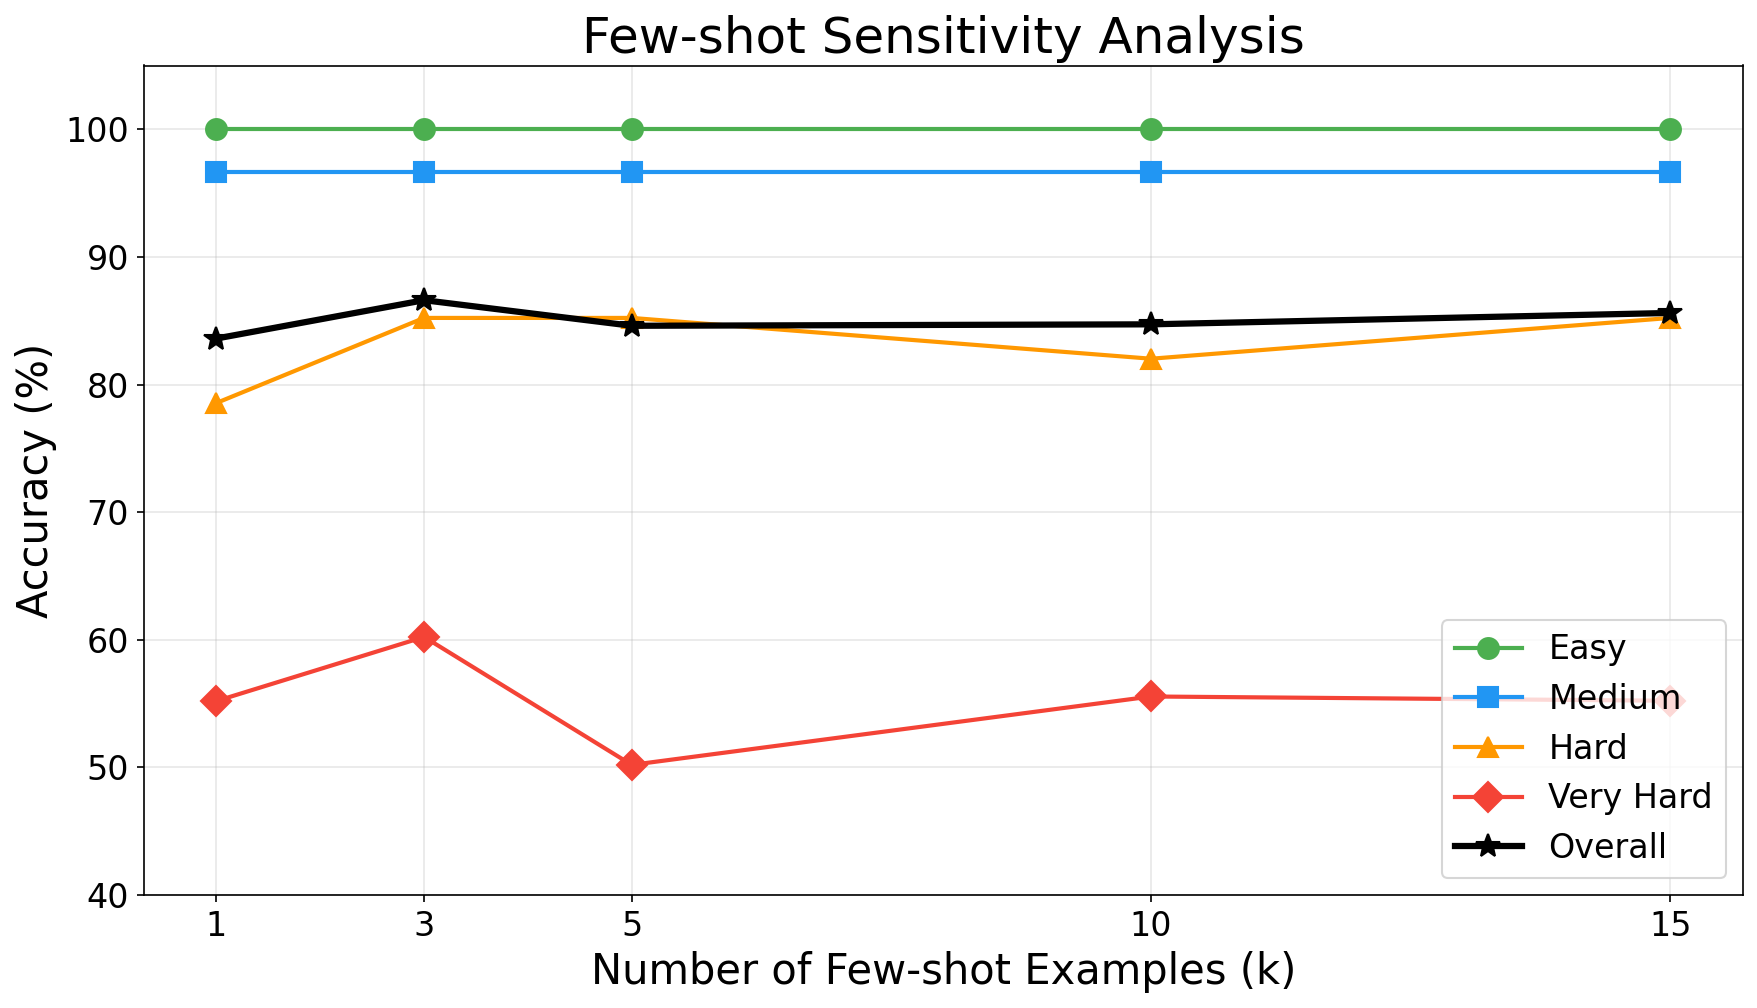
\includegraphics[width=\linewidth]{figures/fewshot_sensitivity.png}
\caption{少数ショット数 $k$ の関数としての難易度層ごとの精度。
Easy/Medium 層は $k$ によらず飽和し、
VH 層は $k=3$ と $k=15$ で最大（88.4\%）となる。}
\label{fig:fewshot_k}
\end{minipage}\hfill
\begin{minipage}[t]{0.40\columnwidth}
\centering
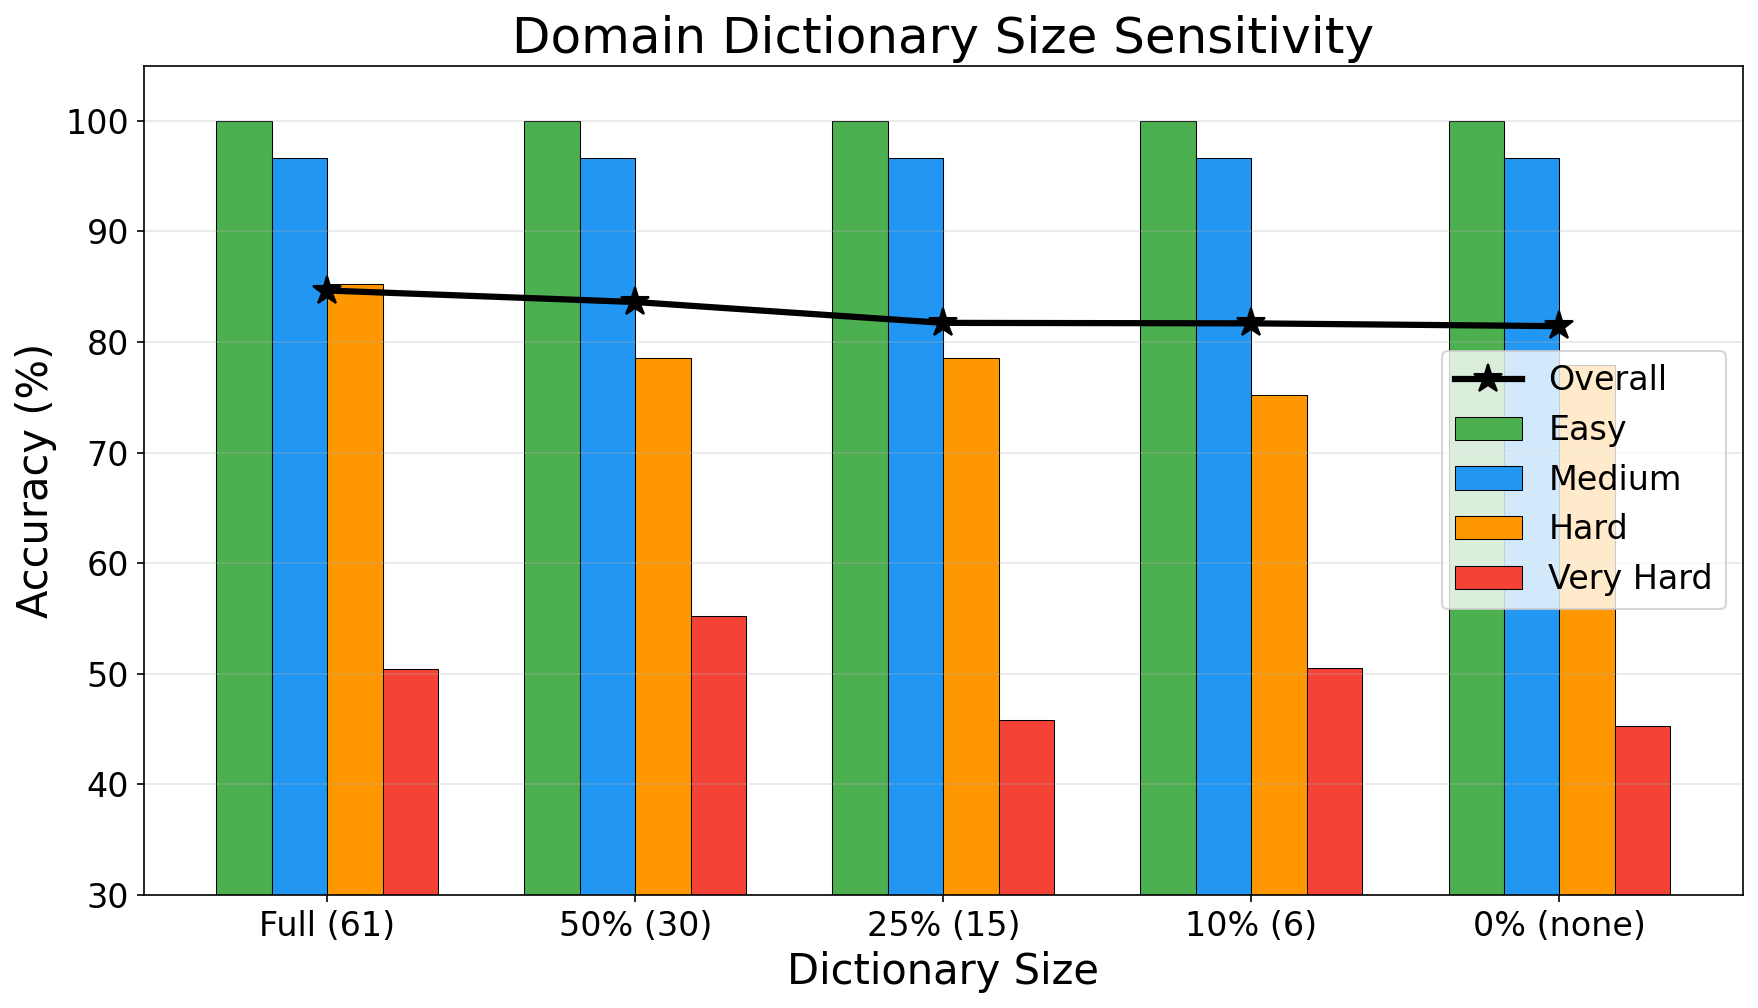
\includegraphics[width=\linewidth]{figures/dict_sensitivity.png}
\caption{ドメイン辞書サイズと難易度層ごとの精度の関係。
辞書サイズの影響はVH層で最も大きい。}
\label{fig:dict_size}
\end{minipage}
\end{figure}


\subsection{LLMモデルの影響（詳細）}

設定と解釈はセクション~\ref{sec:model_comparison}に示した。表~\ref{tab:model_comp}・図~\ref{fig:model_comp}はGPT-5.5（表~\ref{tab:ablation}のfull条件、5ラン平均）とGPT-4o（別の単一ラン）の比較である。

\begin{table}[htbp]
\centering
\caption{LLMモデルの比較。GPT-5.5行は表~\ref{tab:ablation}のfull条件（5ラン平均）、GPT-4o行は別の単一ランで測定した。全体値は未丸め値から算出しており、表示された層別値の加重平均と末尾桁が一致しない場合がある。
GPT-4oはレイテンシが短く、全体・VHともGPT-5.5のfull（5ラン平均）と近い水準を示した（単一ラン比較のため統計的同等性は評価していない）；レイテンシは測定条件が異なるため
表~\ref{tab:fewshot_k} とは直接比較できない。}
\label{tab:model_comp}
\footnotesize
\begin{tabular}{@{}lrrrrrr@{}}
\toprule
モデル & 全体 & Easy & Medium & Hard & VH & レイテンシ (s) \\
\midrule
GPT-5.5 & 92.5 & 99.8 & 96.7 & 86.8 & 87.5 & 30.9 \\
GPT-4o  & 91.7 & 100.0 & 93.3 & 91.8 & 81.0 &  2.1 \\
\bottomrule
\end{tabular}
\end{table}

\begin{figure}[htbp]
\centering
\begin{minipage}[t]{0.32\columnwidth}
\centering
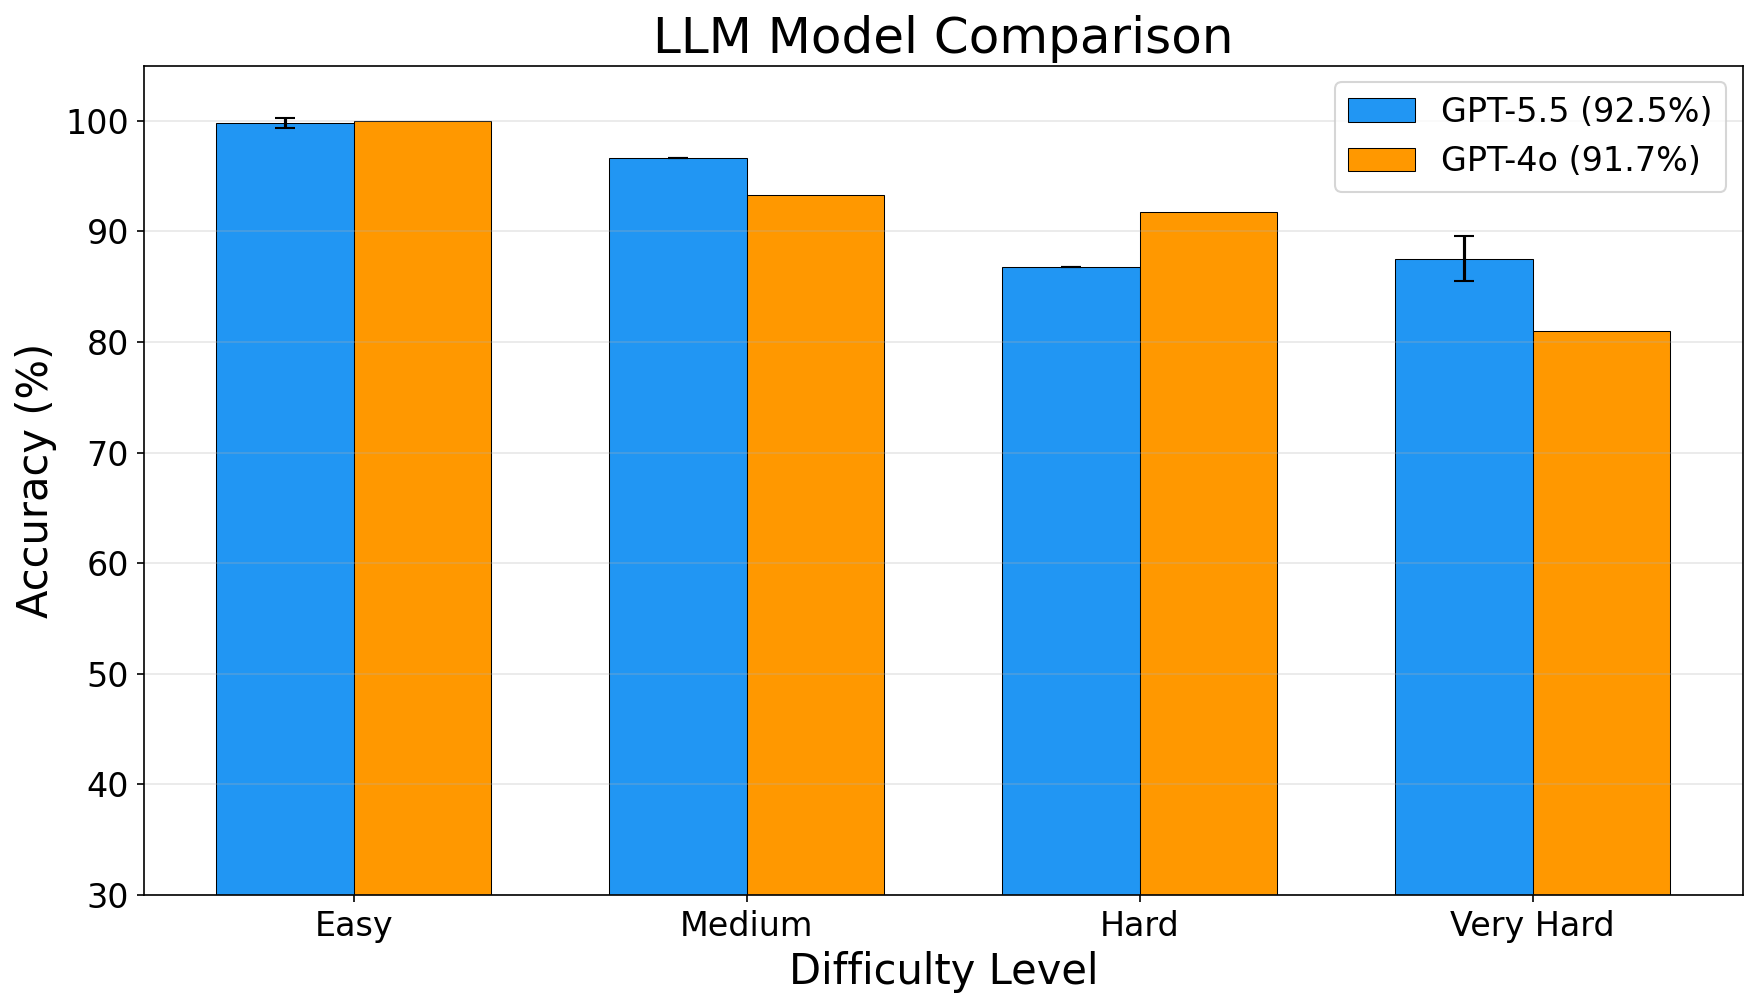
\includegraphics[width=\linewidth]{figures/model_comparison.png}
\caption{難易度層ごとのGPT-5.5とGPT-4oの精度比較。
全体・各層とも差は小さく、GPT-4oはGPT-5.5のfull（5ラン平均）と近い水準を示した（単一ラン比較のため統計的同等性は評価していない）。}
\label{fig:model_comp}
\end{minipage}\hfill
\begin{minipage}[t]{0.32\columnwidth}
\centering
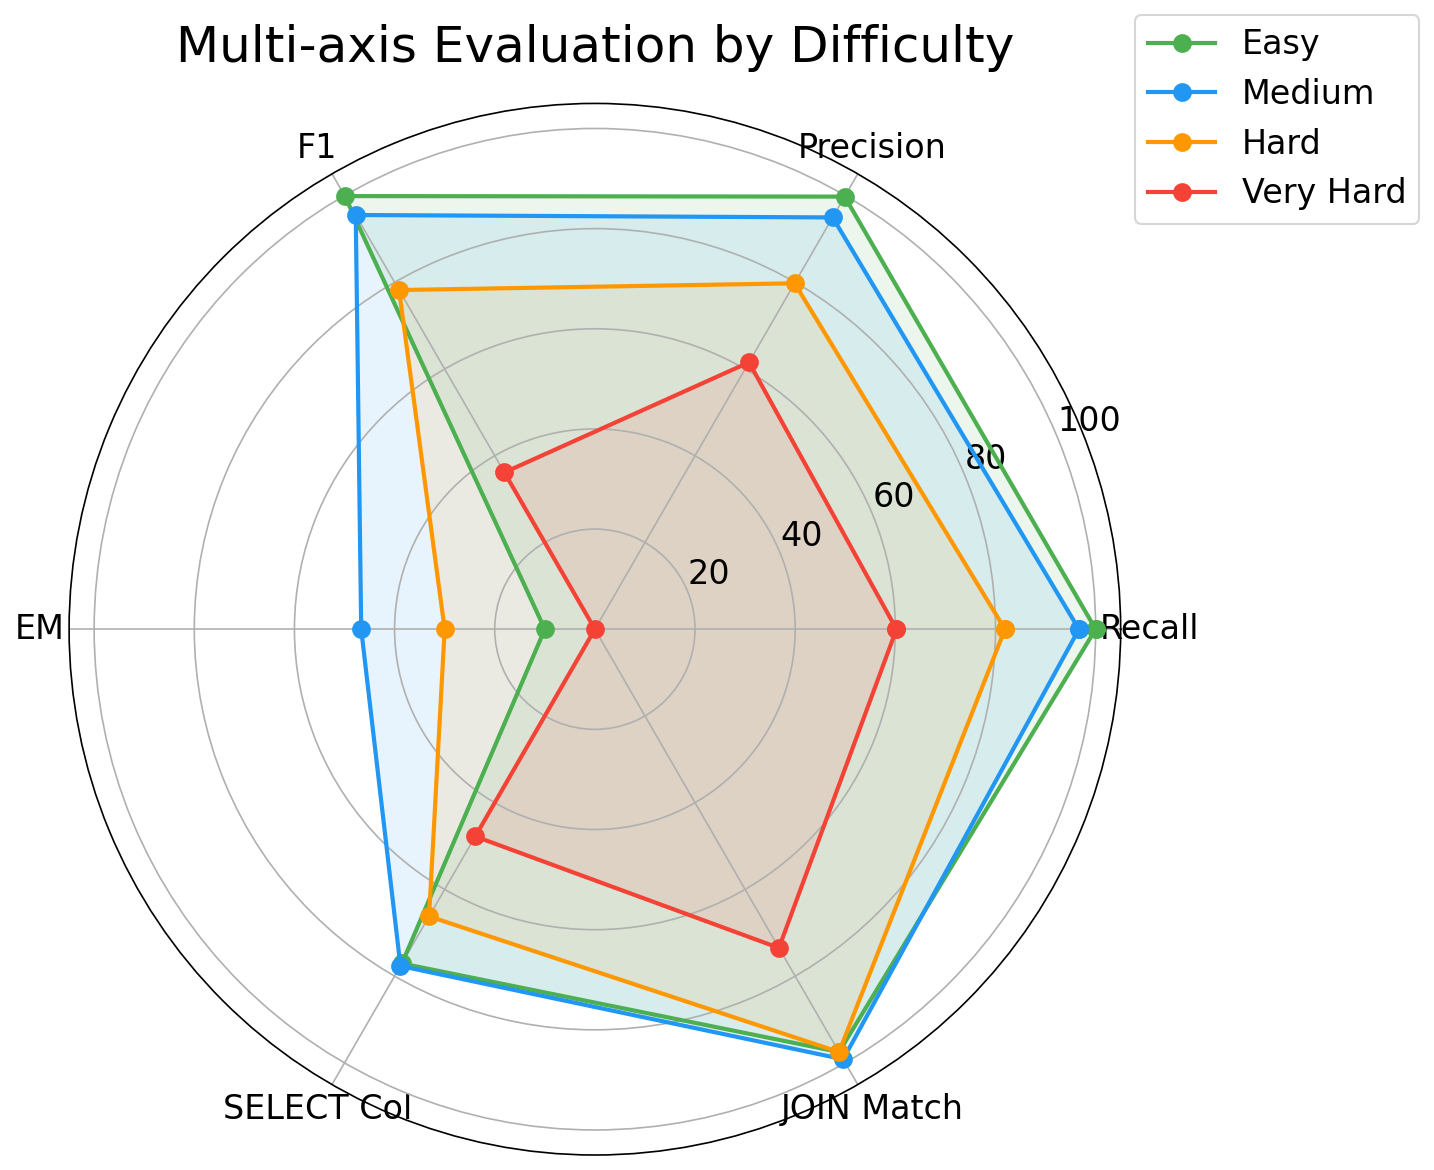
\includegraphics[width=\linewidth]{figures/multiaxis_radar.png}
\caption{難易度層ごとのマルチ軸評価レーダーチャート。
構文と実行の有効性はすべての層で100\%である。
VH層は厳密な完全結果集合一致（Exact軸）が1.6\%と低いが、77.2\%のリコールは多くの部分的に正しい結果を示している。}
\label{fig:radar}
\end{minipage}\hfill
\begin{minipage}[t]{0.32\columnwidth}
\centering

\includegraphics[width=\linewidth]{figures/error_distribution.png}
\caption{保存されたfull条件ラン（245クエリ多軸評価ラン）でリコール0.8未満だった39件における誤差タイプの分布。1ケースに複数の誤差タイプを付与し得るため、ラベルの合計（66）はケース数（39）を上回る。}
\label{fig:error_dist}
\end{minipage}
\end{figure}


\subsection{失敗ケースの内訳分析}

図~\ref{fig:error_dist}は、保存されたfull条件ラン（245クエリ多軸評価ラン）でリコールが0.8未満であった39クエリ（Very Hard 17・Hard 15・Medium 5・Easy 2；セクション~\ref{sec:error_analysis}）における誤差タイプの分布を示す（誤ったカラム選択24、JOIN不一致24、GROUP BY欠如14、値不一致4）。誤ったカラム選択とJOIN不一致が主要であり、ここでのJOIN不一致はゴールドが参照するテーブルの一部が生成SQLに欠けること（主に導出計算用参照テーブルや特性ピボット用JOINの欠落）を意味し、FKに基づかない不正JOINではない（表~\ref{tab:error_analysis}）。失敗は高難易度層に集中し、スキーマグラフが正しいJOINパスを提供していても、LLMが導出量や複合スコア式を含むSELECT句を正確に構成できないケースが残る。


\subsection{SQLインジェクションと安全性テストの入力別結果}

SQLGuardの15の検証項目（セクション~\ref{sec:sqlguard}）は複数の脅威ベクトルに対する深層防御を提供する。禁止キーワードの検出は正規表現ベースであり、テーブルのホワイトリストはスキーマメタデータから自動生成される。

\begin{table}[htbp]
  \centering
  \caption{SQLインジェクションと安全性テスト結果（すべて安全に処理された）。}
  \label{tab:injection_results}
  \footnotesize
  \begin{tabularx}{\linewidth}{lXl}
    \toprule
    ID & 入力 & アクション \\
    \midrule
    E01 & \texttt{DROP TABLE material\_entry;} & ブロック: DROPキーワード \\
    E02 & \texttt{SELECT *; DELETE FROM composition;} & ブロック: マルチステートメント + DELETE \\
    E03 & L1$_2$化合物; \texttt{DROP TABLE structure;} & ブロック: マルチステートメント + DROP \\
    E04 & \texttt{SELECT * FROM secret\_passwords} & ブロック: 不正なテーブル \\
    E05 & \texttt{INSERT INTO material\_entry ...} & ブロック: INSERTキーワード \\
    F01 & \texttt{SELECT entry\_id FROM material\_entry} & LIMIT自動追加（サニタイズ済み） \\
    F02 & \texttt{UPDATE material\_entry SET ...} & ブロック: UPDATEキーワード \\
    \bottomrule
  \end{tabularx}
\end{table}

\subsection{採点方式の監査}
\label{sec:sup_scoring_audit}

本文セクション~\ref{sec:metrics}に述べた採点プロトコルの寛容性（共通列射影・列位置フォールバック・0行一致への満点付与・順序と多重度の無視）の影響を、保存済み評価結果（生成SQL付き保存ラン）に対して同梱の監査スクリプトで定量化した。監査スクリプトは起動時に、現行方針（historical）で同梱のper-queryスコアを完全再現できることを4データセットすべてで自己検査する（LLM・APIキー不要）。表~\ref{tab:scoring_audit}に採点方針別の値を示す。

\begin{table}[htbp]
  \centering
  \caption{採点方針別の実行再現率（\%）。historical＝本文の採点方式。require all＝全ゴールド列の存在を要求。no positional＝列位置フォールバック無効。drop empty＝ゴールド0行クエリを分母から除外。multiset＝行の重複度を照合。exact＝厳密な完全結果集合一致（ゴールド列リスト、行の多重集合を照合し、行順序は期待結果の\texttt{semantic\_ordered}契約が真のクエリ（主評価では245件中39件）に限り照合）。ordered＝exactとは母集団の異なる別指標で、各データセットの\texttt{ORDER BY}付きゴールドクエリ（主評価では234件）に対する順序照合Recall；この列の定義は\texttt{semantic\_ordered}契約とは独立である。緩い完全一致（共通列射影上でPrecision=Recall=1；78.0\%）は本表の列には含めず、同梱の\texttt{scoring\_audit.json}に\texttt{common\_column\_exact\_overlap\_pct}として収録する。同JSONは、全ゴールド列必須・位置フォールバック無効・ゴールド0行除外・多重集合照合を同時に課す（順序照合のみ課さない）strict方針（主評価25.5\%、$n=241$）も収録する。いずれも生成SQL付き保存ラン（main: 245クエリ、historical Recall 86.1\%の単一ラン）に基づく。}
  \label{tab:scoring_audit}
  \footnotesize
  \begin{tabular}{@{}lrrrrrrr@{}}
    \toprule
    データセット & hist. & req.\ all & no pos. & drop empty & multiset & exact & ordered \\
    \midrule
    主評価 (245) & 86.1 & 26.3 & 82.8 & 86.3 & 83.9 & 10.6 & 54.3 \\
    独立設計 (100) & 81.5 & 4.0 & 76.4 & 81.9 & 80.3 & 1.0 & 50.4 \\
    一般化B (20) & 85.0 & 40.0 & 70.0 & 85.0 & 85.0 & 15.0 & 66.5 \\
    一般化C (20) & 80.0 & 30.0 & 60.0 & 80.0 & 77.0 & 20.0 & 57.4 \\
    \bottomrule
  \end{tabular}
\end{table}

解釈上の注意を3点述べる。第一に、「require all」の低下（主評価26.3\%）は影響の上限であり、ゴールドSQLが補助列（\texttt{entry\_id}等）を含む設計に起因する部分が大きく、報告値としては採用しない。実質的に効くのは「recall=1.0だがゴールド1列のみで比較された」クエリ（主評価33件・独立設計18件・一般化B 5件・C 4件）である。ゴールドSQL修正前の保存ランに対する同種の目視監査で明確な過大評価と判定された4件（\texttt{q\_hard\_021}・\texttt{q\_vhard\_009}・\texttt{q\_vhard\_018}・\texttt{q\_vhard\_020}、いずれも導出計算系）については、ゴールド修正後の再評価でも別途、全ゴールド列を必須とする厳格採点を適用した監査（アブレーション5ラン$\times$7条件の35生成/クエリ）を実施し、記録された寛容採点の平均リコール（各クエリの35生成平均で0.686--1.00）に対し厳格採点では4件とも0.0であること、すなわち生成SQLが要求された導出計算を依然実行していないことを確認した（監査結果として同梱）。この厳格値は本文の主要指標には算入せず、監査結果として分離して報告する。第二に、順序照合（ordered）の低値の多くはゴールドSQLが決定性確保のために付す\texttt{ORDER BY}に由来する（主評価では\texttt{ORDER BY}付きゴールド234件に対する順序照合Recallが54.3\%）。この列はexact列とは別指標であり、exactが行順序を照合するのは質問文自体が順序付き回答を要求する\texttt{semantic\_ordered}契約付きの39件のみである（残る195件の\texttt{ORDER BY}は決定性確保のためのものであり、exactでは順序を課さない）。ランキングを要する問いでは行集合が正しくても順位が誤り得ることに注意が必要である。第三に、これらはいずれも同一の保存ランに対する採点方式の感度分析であり、本文の主要値（245クエリ多軸評価のRecall 86.1\%等）の再測定ではない。

% =====================================================================
\section{考察の補足}
\label{sec:sup_discussion_details}

\subsection{CTE評価の5カテゴリと条件別精度}
\label{sec:cte_evaluation}

few-shot例でカバーされた既知5パターンは、シンプルCTE（導出量計算）・CTE＋フィルター・CTE＋集約・マルチステージCTE（2段階以上）・CTE＋クロスカラム比較の5カテゴリをカバーする。表~\ref{tab:cte_results}は、CTEマルチステップ計算15クエリ（既知5パターン＋新規10ゼロショットパターン；いずれも主評価245クエリに含まれ、既知5はアブレーション用100クエリサブセット内、新規10はサブセット外）の精度を示している。

\begin{table}[htbp]
\centering
\caption{CTEマルチステップ計算クエリの精度。上段はfull条件の15クエリ（既知5＋新規10）、下段は既知5パターンに対するアブレーション条件別精度（5ラン平均）である。few-shot例でカバーされた既知5パターンは100\%を維持する一方、例のない新規10パターンは59.0\%にとどまり、マルチステップ計算サポートの範囲がfew-shot例のパターンカバレッジに規定されることを示す。}
\label{tab:cte_results}
\footnotesize
\begin{tabular}[t]{@{}lrr@{}}
\toprule
サブセット & $n$ & 実行再現率 \\
\midrule
既知5パターン（few-shot例あり） & 5 & 100.0\% \\
新規10パターン（ゼロショット） & 10 & 59.0\% \\
\midrule
全体 & 15 & 72.7\% \\
\bottomrule
\end{tabular}\hspace{2em}
\begin{tabular}[t]{@{}lrr@{}}
\toprule
\multicolumn{3}{@{}l}{条件別精度（既知5パターン、5ラン平均）} \\
条件 & $n$ & 実行再現率 \\
\midrule
full & 5 & 100.0\% \\
no\_fewshot & 5 & 60.0\% \\
no\_dict & 5 & 80.0\% \\
no\_reranker & 5 & 100.0\% \\
no\_guard & 5 & 100.0\% \\
no\_nbest & 5 & 96.0\% \\
no\_graph & 5 & 100.0\% \\
\bottomrule
\end{tabular}
\end{table}


\subsection{一般化評価バリアントの詳細}

表~\ref{tab:transfer_eval}の各バリアントの定義と難易度別の内訳を示す（解釈上の注意はセクション~\ref{sec:transfer_eval}）。

バリアントA---5プロトタイプ横断クエリ。主評価と同一の検証DB（B2/NaCl/NiAs/BiF$_3$を含む）に対し、非L1$_2$プロトタイプを対象とするクエリを含む20の評価クエリ（\texttt{q\_proto\_*}）を実行した。この20クエリは主評価245クエリの部分集合であり（表~\ref{tab:main_partition}）、独立した一般化試験のコーパスではない。結果は同一問題の別ランとして100.0\%（全難易度で100\%）であり、主評価の単一ラン内では同20クエリは85.0\%であった（差はラン間変動を含む）。

バリアントB---OQMD風のリネーム。すべてのテーブルとカラム名が変更されたOQMD風のフラット5テーブルスキーマ（\texttt{oqmd\_entries}, \texttt{oqmd\_element\_ratios}, \texttt{oqmd\_formation\_energies}, \texttt{oqmd\_reference\_states}, \texttt{oqmd\_elements}）に対し、少数ショット例は元のスキーマのまま提示してSQLパターンのみを再利用するよう指示した。結果は85.0\%（Easy 100\% / Medium 83.3\% / Hard 80.0\% / Very Hard 66.7\%）であった。

バリアントC---識別子難読化。転送DB内のすべてのスキーマ識別子を、FK関係を保持したままランダムな英単語に置き換えた。実行再現率は80.0\%（Easy 100\% / Medium 83.3\% / Hard 60.0\% / Very Hard 66.7\%；平均レイテンシ34.3\,s）であり、意味のある識別子名が失われても一定の性能を維持したが、この実験だけから「FKトポロジーのみで十分」とは結論しない。

バリアントD---マテリアルズプロジェクト風スキーマ。実際のMaterials Project RESTデータから27の二元系（299エントリ）を取得し、3テーブルPostgreSQLスキーマ（\texttt{mp\_entries}, \texttt{mp\_elements}, \texttt{mp\_element\_ratios}）を構築した。15の日本語クエリに対し、MPスキーマ用の8件のfew-shot例とMP専用プロンプトを与えたが、パイプラインコード自体は変更していない。実行再現率は93.3\%（Easy/Medium/Hard 100\%、Very Hard 66.7\%）であった。

\subsection{列間比較クエリの3パターン}
\label{sec:sup_column_comparison}

セクション~\ref{sec:column_comparison}で述べた列間比較クエリについて、少数ショット例がカバーする3パターンとSQL断片を示す。
\begin{enumerate}  
  \item テーブル内比較：  
    同じテーブル内の2つの列の直接比較。  
    例：\texttt{formation\_energy\_per\_atom < energy\_above\_hull}（\texttt{phase\_stability}テーブル内）；  
    \texttt{bulk\_modulus\_vrh > 2.0 * shear\_modulus\_vrh}（\texttt{elastic\_tensor}テーブル内、Pugh延性メトリック）。  
  \item テーブル間比較：  
    JOINを介して異なるテーブルの列を比較。  
    例：\texttt{thermal\_property.debye\_temperature\_k > magnetic\_property.curie\_temperature\_k}；  
    総磁化対絶対生成エネルギー。  
  \item 集約関数を用いた比較：  
    GROUP BY--HAVINGと組み合わせて、構成要素間の電気陰性度差などの導出量に対する閾値評価を行う。  
    例：\texttt{HAVING MAX(electronegativity) - MIN(electronegativity) > 0.5}。  
\end{enumerate}

\subsection{あいまい・矛盾クエリの例}
\label{sec:sup_ambiguous}

実際のユーザーが投入し得るあいまい・矛盾クエリの例として次のようなものが挙げられる：(i)~「NiAl の組成比で L1$_2$ 構造のものを出してほしい」（NiAl は 1:1 組成の B2 型であり、1:3 組成の L1$_2$ とは前提が矛盾する）、(ii)~「安定な化合物を出して」（凸包距離か生成エンタルピーの符号か、ユーザーが基準を指定しない限り一義的でない。なお本評価ではセクション~\ref{sec:query_design}の操作的定義$E_\text{hull} \leq 0.001$~eV/atomに固定している）、(iii)~「生成エンタルピーが 0.5\,eV より大きい安定化合物」（安定性は負の生成エンタルピーを意味するため閾値と矛盾する）、(iv)~「融点が 2{,}000\,K 以上の L1$_2$ 化合物」（スキーマに存在しない属性への問い）、(v)~「$\gamma$ 相の合金を出して」（鉄鋼の $\gamma$（fcc）か Ni 基超合金の $\gamma'$ かが不明な多義語）、(vi)~「一番多い元素は？」（材料数ベースか組成比ベースかの集計単位が不明）、(vii)~「D0$_{19}$ 構造の化合物」（検証データベースに存在しないプロトタイプ）。これらは条件の欠落・矛盾・スキーマ外参照という異なる失敗様式を代表する。

\section{再現ワークフロー}
\label{sec:sup_workflow}

配布パッケージの再現ワークフローは、データ準備・DB構築・評価データセット（ステップ1--3）、LLM評価実行（ステップ4）、統計解析・集計・図表生成（ステップ5--6）、数値整合検証と原稿コンパイル（ステップ7）から成る。ステップ4のみがLLM APIキーを必要とし非決定的であるため、論文の全掲載数値と図6点はパッケージに保存された評価出力から決定的に再生成される：ステップ5では各クエリの5ラン平均（$n=100$）に対するWilcoxon符号順位統計量の両側全符号置換検定（同順位は中央順位で処理；言語評価（セクション~\ref{sec:language_eval}）と同一の実装を共有し、SciPyのバージョンに依存しない）・Holm補正・クエリ単位ブートストラップ95\%CI（20{,}000再標本）を算出し、ステップ6の結果集約プログラムが単一情報源（SSOT）を生成したうえで図生成プログラムがSSOTのみから図を出力する。結果集約プログラムは冒頭でユニットテストスイート（166件）を実行して1件でも失敗すれば停止し（テストゲート）、ステップ7の数値整合検証プログラムはSSOTと原稿TeX中の掲載値を突き合わせて不一致があれば失敗する。各ステップに対応するスクリプト・入出力ファイル・保存済み評価出力と論文の表・図との対応表は、同梱の\texttt{MANIFEST.md}および\texttt{README\_SQL.md}に記載した。

\end{document}
